\documentclass[12pt,a4paper]{report}

% ==============================================================================
% PACKAGES & SYSTEM CONFIGURATION
% ==============================================================================
\usepackage[utf8]{inputenc}
\usepackage[T1]{fontenc}
\usepackage{lmodern}
\usepackage[left=1.25in, right=1.0in, top=1.0in, bottom=1.0in]{geometry}
\usepackage{setspace}
\onehalfspacing

\usepackage{amsmath, amssymb, amsfonts}
\usepackage{graphicx}
\usepackage{booktabs}
\usepackage{tabularx}
\usepackage{longtable}
\usepackage{multirow}
\usepackage{array}
\usepackage{float}
\usepackage{caption}
\usepackage{subcaption}
\usepackage{enumitem}
\usepackage{xcolor}
\usepackage{listings}
\usepackage{algorithm}
\usepackage{algpseudocode}
\usepackage{tikz}
\usetikzlibrary{shapes.geometric, arrows, arrows.meta, positioning, fit, calc}
\usepackage{pgfplots}
\pgfplotsset{compat=1.18}

\usepackage{fancyhdr}
\usepackage{titlesec}
\usepackage[colorlinks=true, linkcolor=blue!70!black, citecolor=green!50!black, urlcolor=blue!80!black]{hyperref}

% Page numbering and header style
\pagestyle{fancy}
\fancyhf{}
\fancyfoot[C]{\thepage}
\renewcommand{\headrulewidth}{0pt}

% Title formats
\titleformat{\chapter}[display]
  {\normalfont\huge\bfseries\centering}{\chaptertitlename\ \thechapter}{15pt}{\Huge}
\titlespacing*{\chapter}{0pt}{20pt}{30pt}

% Code listing configuration
\definecolor{codegreen}{rgb}{0,0.6,0}
\definecolor{codegray}{rgb}{0.5,0.5,0.5}
\definecolor{codepurple}{rgb}{0.58,0,0.82}
\definecolor{backcolour}{rgb}{0.96,0.96,0.98}

\lstdefinestyle{clinexuscode}{
    backgroundcolor=\color{backcolour},   
    commentstyle=\color{codegreen}\itshape,
    keywordstyle=\color{blue}\bfseries,
    numberstyle=\tiny\color{codegray},
    stringstyle=\color{codepurple},
    basicstyle=\ttfamily\footnotesize,
    breakatwhitespace=false,         
    breaklines=true,                 
    captionpos=b,                    
    keepspaces=true,                 
    numbers=left,                    
    numbersep=6pt,                  
    showspaces=false,                
    showstringspaces=false,
    showtabs=false,                  
    tabsize=2,
    frame=single,
    rulecolor=\color{black!20}
}
\lstset{style=clinexuscode}

% ==============================================================================
% DOCUMENT BEGINS
% ==============================================================================
\begin{document}

% ------------------------------------------------------------------------------
% 1. COVER / TITLE PAGE
% ------------------------------------------------------------------------------
\begin{titlepage}
\begin{center}
    \vspace*{0.5cm}
    
    {\fontsize{20pt}{24pt}\selectfont \textbf{CLINEXUS: AN EXPLAINABLE MULTI-AGENT CLINICAL INTELLIGENCE PLATFORM FOR CLINICAL DECISION ASSISTANCE}}\\[1.8cm]
    
    {\fontsize{13pt}{16pt}\selectfont A Report on Major Project Part 1\\
    submitted in partial fulfillment of the requirements for\\
    the award of the degree of}\\[0.6cm]
    
    {\fontsize{16pt}{20pt}\selectfont \textbf{Bachelor of Engineering}}\\[0.3cm]
    {\fontsize{13pt}{16pt}\selectfont in}\\[0.3cm]
    {\fontsize{15pt}{18pt}\selectfont \textbf{Artificial Intelligence and Data Science}}\\[1.2cm]
    
    {\fontsize{13pt}{16pt}\selectfont By}\\[0.4cm]
    {\fontsize{14pt}{17pt}\selectfont \textbf{D. Sai Charan (1601-23-771-105)}}\\[0.2cm]
    {\fontsize{14pt}{17pt}\selectfont \textbf{K. V. N. S. Vishnu Vardhan (1601-23-771-113)}}\\[0.2cm]
    {\fontsize{14pt}{17pt}\selectfont \textbf{L. Sai Santhosh (1601-23-771-116)}}\\[1.2cm]
    
    {\fontsize{12pt}{15pt}\selectfont Under the esteemed guidance of}\\[0.3cm]
    {\fontsize{14pt}{17pt}\selectfont \textbf{Mrs. Swathi Tejah Yalla}}\\[0.15cm]
    {\fontsize{12pt}{15pt}\selectfont Assistant Professor}\\[1.2cm]
    
    \begin{figure}[H]
        \centering
        \fbox{\parbox[c][2.2cm][c]{2.2cm}{\centering \textbf{INSTITUTE LOGO}\\ \scriptsize (CBIT, Hyderabad)}}
    \end{figure}
    \vspace{0.4cm}
    
    {\fontsize{13pt}{16pt}\selectfont \textbf{DEPARTMENT OF ARTIFICIAL INTELLIGENCE AND DATA SCIENCE}}\\[0.2cm]
    {\fontsize{14pt}{17pt}\selectfont \textbf{CHAITANYA BHARATHI INSTITUTE OF TECHNOLOGY (A)}}\\[0.2cm]
    {\fontsize{12pt}{15pt}\selectfont \textbf{HYDERABAD -- 500075}}\\[0.2cm]
    {\fontsize{12pt}{15pt}\selectfont \textbf{NOVEMBER 2026}}
\end{center}
\end{titlepage}

% Front matter page numbering (Roman)
\pagenumbering{roman}
\setcounter{page}{2}

% ------------------------------------------------------------------------------
% 2. INSTITUTE & DEPARTMENT VISION AND MISSION
% ------------------------------------------------------------------------------
\newpage
\begin{center}
    \fbox{\parbox[c][1.8cm][c]{1.8cm}{\centering \scriptsize CBIT LOGO}}
    \vspace{0.4cm}
    
    \textbf{\large DEPARTMENT OF ARTIFICIAL INTELLIGENCE AND DATA SCIENCE}\\[0.1cm]
    \textbf{\large CHAITANYA BHARATHI INSTITUTE OF TECHNOLOGY (A)}\\[0.1cm]
    \textbf{\large HYDERABAD -- 500075}\\[1.0cm]
    
    \textbf{\Large INSTITUTE VISION}\\[0.4cm]
    \textit{``To be the center of excellence in technical education and research''.}\\[1.0cm]
    
    \textbf{\Large INSTITUTE MISSION}\\[0.4cm]
    \textit{``To address the emerging needs through quality technical education and advanced research''.}\\[1.2cm]
    
    \textbf{\Large DEPARTMENT VISION}\\[0.4cm]
    \textit{``To be a globally recognized center of excellence in the field of Artificial Intelligence and Data Science that produces innovative pioneers and research experts capable of addressing complex real-world challenges and contributing to the socio-economic development of the nation.''}\\[1.0cm]
    
    \textbf{\Large DEPARTMENT MISSION}\\[0.4cm]
\end{center}

\begin{enumerate}[label=\textbf{\arabic*.}]
    \item To provide cutting-edge education in the field of Artificial Intelligence and Data Science that is rooted in ethical and moral values.
    \item To establish strong partnerships with industries and research organizations in the field of Artificial Intelligence and Data Science, and to excel in the emerging areas of research by creating innovative solutions.
    \item To cultivate a strong sense of social responsibility among students, fostering their inclination to utilize their knowledge and skills for the betterment of society.
    \item To motivate and mentor students to become trailblazers in Artificial Intelligence and Data Science, and develop an entrepreneurial mindset that nurtures innovation and creativity.
\end{enumerate}

% ------------------------------------------------------------------------------
% 3. DECLARATION CERTIFICATE
% ------------------------------------------------------------------------------
\newpage
\begin{center}
    \fbox{\parbox[c][1.8cm][c]{1.8cm}{\centering \scriptsize CBIT LOGO}}
    \vspace{0.4cm}
    
    \textbf{\large DEPARTMENT OF ARTIFICIAL INTELLIGENCE AND DATA SCIENCE}\\[0.1cm]
    \textbf{\large CHAITANYA BHARATHI INSTITUTE OF TECHNOLOGY (A)}\\[0.1cm]
    \textbf{\large HYDERABAD -- 500075}\\[1.0cm]
    
    \textbf{\Large DECLARATION CERTIFICATE}\\[1.0cm]
\end{center}

We hereby declare that the project titled \textbf{``CLINEXUS: An Explainable Multi-Agent Clinical Intelligence Platform for Clinical Decision Assistance''} submitted by us to the Department of Artificial Intelligence and Data Science, \textbf{CHAITANYA BHARATHI INSTITUTE OF TECHNOLOGY, HYDERABAD} in partial fulfillment of the requirements for the award of \textbf{Bachelor of Engineering} is a bonafide record of the work carried out by us under the supervision of \textbf{Mrs. Swathi Tejah Yalla}, Assistant Professor. 

We hereby declare that the work presented in this project has not been submitted, either in whole or in part, and will not be submitted to this or any other institute or university for the award of any other degree.

\vspace{3.5cm}

\begin{flushright}
    \textbf{Project Associates}\\[0.5cm]
    \textbf{D. Sai Charan (1601-23-771-105)}\\[0.2cm]
    \textbf{K. V. N. S. Vishnu Vardhan (1601-23-771-113)}\\[0.2cm]
    \textbf{L. Sai Santhosh (1601-23-771-116)}\\
\end{flushright}

% ------------------------------------------------------------------------------
% 4. BONAFIDE CERTIFICATE
% ------------------------------------------------------------------------------
\newpage
\begin{center}
    \fbox{\parbox[c][1.8cm][c]{1.8cm}{\centering \scriptsize CBIT LOGO}}
    \vspace{0.4cm}
    
    \textbf{\large DEPARTMENT OF ARTIFICIAL INTELLIGENCE AND DATA SCIENCE}\\[0.1cm]
    \textbf{\large CHAITANYA BHARATHI INSTITUTE OF TECHNOLOGY (A)}\\[0.1cm]
    \textbf{\large HYDERABAD -- 500075}\\[1.0cm]
    
    \textbf{\Large BONAFIDE CERTIFICATE}\\[1.0cm]
\end{center}

This is to certify that the project titled \textbf{``CLINEXUS: An Explainable Multi-Agent Clinical Intelligence Platform for Clinical Decision Assistance''} is a bonafide record of the work done by:

\begin{center}
    \textbf{D. Sai Charan (1601-23-771-105)}\\[0.15cm]
    \textbf{K. V. N. S. Vishnu Vardhan (1601-23-771-113)}\\[0.15cm]
    \textbf{L. Sai Santhosh (1601-23-771-116)}\\
\end{center}

\noindent in partial fulfillment of the requirements for the award of the degree of \textbf{Bachelor of Engineering in Artificial Intelligence and Data Science} to the \textbf{CHAITANYA BHARATHI INSTITUTE OF TECHNOLOGY, HYDERABAD} carried out under my guidance and supervision during the academic year 2026--27. The results presented in this project report have not been submitted to any other university or Institute for the award of any other degree.

\vspace{2.5cm}

\noindent
\begin{tabular*}{\textwidth}{@{\extracolsep{\fill}}cc}
    \textbf{Mrs. Swathi Tejah Yalla} & \textbf{Prof. K. Radhika} \\
    Guide & Head of the Department
\end{tabular*}

\vspace{2.0cm}

\noindent Submitted for Semester Major-Project Part 1 viva-voce examination held on \underline{\hspace{4cm}}

\vspace{1.5cm}

\noindent
\begin{tabular*}{\textwidth}{@{\extracolsep{\fill}}cc}
    \textbf{Examiner-1} & \textbf{Examiner-2}
\end{tabular*}

% ------------------------------------------------------------------------------
% 5. ACKNOWLEDGEMENTS
% ------------------------------------------------------------------------------
\newpage
\begin{center}
    \textbf{\Large ACKNOWLEDGEMENTS}\\[1.0cm]
\end{center}

We would like to express our deepest gratitude to the people who guided us through this course and without whom this project would not have reached its present form.

Our heartfelt thanks to \textbf{Mrs. Swathi Tejah Yalla}, Assistant Professor, Department of Artificial Intelligence and Data Science, for her expert guidance throughout this project, insightful technical suggestions, and continuous supervision. Her patience, technical rigor, and encouraging attitude have always been, and will continue to be, an abiding source of inspiration to us.

Our heartfelt thanks to \textbf{Prof. K. Radhika}, Head of the Department of Artificial Intelligence and Data Science, for her encouragement and for allowing us to use the computing facilities, laboratories, and resources of the department.

We also express our sincere thanks to the respected Principal and Management of Chaitanya Bharathi Institute of Technology for providing an environment conducive to research and academic excellence.

We also thank the faculty and staff of the Department of Artificial Intelligence and Data Science, our parents, and our friends for their unwavering support, moral encouragement, and assistance throughout the execution of this project.

\vspace{1.0cm}
\noindent \textbf{Use of Generative AI Tools.} AI coding assistants (including Anthropic Claude and Google Gemini) were utilized to aid in drafting and testing backend service modules, generating automated unit test fixtures, validating schema constraints, and assisting with \LaTeX{} formatting from our architectural designs. All generated logic, schema rules, algorithmic flows, and experimental configurations were rigorously verified, independently tested, and validated by the student project associates, who assume full responsibility for the contents of this report.

% ------------------------------------------------------------------------------
% 6. TABLE OF CONTENTS, LIST OF TABLES, LIST OF FIGURES
% ------------------------------------------------------------------------------
\newpage
\tableofcontents

\newpage
\listoftables

\newpage
\listoffigures

% ------------------------------------------------------------------------------
% 7. ABBREVIATIONS & SYMBOLS
% ------------------------------------------------------------------------------
\newpage
\begin{center}
    \textbf{\Large ABBREVIATIONS}\\[0.8cm]
\end{center}

\begin{table}[H]
\centering
\begin{tabularx}{\textwidth}{lX}
\toprule
\textbf{Abbreviation} & \textbf{Expansion} \\
\midrule
AI & Artificial Intelligence \\
BioASQ & Biomedical Semantic Indexing and Question Answering \\
BioBERT & Biomedical Bidirectional Encoder Representations from Transformers \\
CDSS & Clinical Decision Support System \\
EHR & Electronic Health Record \\
FHIR & Fast Healthcare Interoperability Resources \\
FSM & Finite State Machine \\
HITL & Human-in-the-Loop \\
HTTP & Hypertext Transfer Protocol \\
ICD & International Classification of Diseases \\
JSON & JavaScript Object Notation \\
LLM & Large Language Model \\
MAP & Mean Average Precision \\
MCP & Model Context Protocol \\
MeSH & Medical Subject Headings \\
MRR & Mean Reciprocal Rank \\
NCBI & National Center for Biotechnology Information \\
NER & Named Entity Recognition \\
NLI & Natural Language Inference \\
ORM & Object-Relational Mapping \\
PII & Personally Identifiable Information \\
PMID & PubMed Identifier \\
PRISMA & Preferred Reporting Items for Systematic Reviews and Meta-Analyses \\
PROV-O & W3C Provenance Ontology \\
RAG & Retrieval-Augmented Generation \\
RBAC & Role-Based Access Control \\
REST & Representational State Transfer \\
SaMD & Software as a Medical Device \\
SNOMED CT & Systematized Nomenclature of Medicine -- Clinical Terms \\
SQL & Structured Query Language \\
URI & Uniform Resource Identifier \\
UUID & Universally Unique Identifier \\
XAI & Explainable Artificial Intelligence \\
\bottomrule
\end{tabularx}
\end{table}

\newpage
\begin{center}
    \textbf{\Large SYMBOLS}\\[0.8cm]
\end{center}

\begin{table}[H]
\centering
\begin{tabularx}{\textwidth}{lX}
\toprule
\textbf{Symbol} & \textbf{Meaning} \\
\midrule
$\tau$ & Confidence decision threshold for workflow completion ($\tau = 0.65$) \\
$C$ & Composite system confidence score ($C \in [0.0, 1.0]$) \\
$w_1, w_2, w_3, w_4$ & Weights for confidence factors ($0.50, 0.20, 0.15, 0.15$) \\
$S_{\text{claim}}$ & Claim support ratio: $\frac{|\text{SUPPORTED}| + 0.5 \cdot |\text{PARTIALLY\_SUPPORTED}|}{|\text{Material Claims}|}$ \\
$R_{\text{strength}}$ & Scaled retrieval score of top-$k$ retrieved evidence passages \\
$A_{\text{source}}$ & Proportion of available external and internal retrieval sources \\
$I_{\text{comp}}$ & Case clinical information completeness ratio ($1 - \frac{\text{missing}}{\text{required}}$) \\
$k$ & Top-$k$ nearest neighbor retrieval parameter ($k=10$) \\
$P@k$ & Precision at rank cutoff $k$ \\
$R@k$ & Recall at rank cutoff $k$ \\
$AP$ & Average Precision normalized across total ground-truth relevant items $|R|$ \\
$N_{\text{iter}}$ & Optimization feedback iteration index ($N_{\text{iter}} \in \{0, 1, 2, 3\}$) \\
$N_{\text{max}}$ & Hard ceiling of adaptive optimization feedback loops ($N_{\text{max}} = 3$) \\
$h_i$ & Cryptographic hash of audit event $i$, $h_i = \text{SHA-256}(h_{i-1} \parallel \text{event}_i)$ \\
$e$ & Evidence passage unit carrying platform identifier $\text{ev}:\langle\text{source}\rangle:\langle\text{id}\rangle:\langle\text{chunk}\rangle$ \\
\bottomrule
\end{tabularx}
\end{table}

% ------------------------------------------------------------------------------
% 8. SUSTAINABLE DEVELOPMENT GOALS (SDGs) MAPPING
% ------------------------------------------------------------------------------
\newpage
\begin{center}
    \textbf{\Large SUSTAINABLE DEVELOPMENT GOALS (SDGs) MAPPING}\\[0.8cm]
\end{center}

The United Nations Sustainable Development Goals (SDGs) constitute a universal call to action to end poverty, protect the planet, and ensure health and prosperity for all. The \textbf{CLINEXUS} platform directly addresses and supports four critical United Nations Sustainable Development Goals:

\vspace{0.4cm}

\noindent\begin{tabularx}{\textwidth}{m{2.5cm}X}
\toprule
\centering \textbf{Goal} & \textbf{Contribution and Alignment with CLINEXUS} \\
\midrule
\centering \fbox{\parbox[c][1.4cm][c]{2.0cm}{\centering \textbf{SDG 3}\\ \scriptsize Good Health \& Well-Being}} & \textbf{SDG 3 -- Good Health and Well-Being (Target 3.8, 3.b):} Clinicians face heavy diagnostic cognitive workloads and information overload. CLINEXUS empowers medical practitioners with verified, evidence-grounded clinical intelligence, mitigating diagnostic omissions, reducing medical diagnostic errors, and accelerating evidence-based differential assessments for complex patient conditions. \\
\addlinespace[0.4cm]
\centering \fbox{\parbox[c][1.4cm][c]{2.0cm}{\centering \textbf{SDG 9}\\ \scriptsize Industry, Innovation \& Infra}} & \textbf{SDG 9 -- Industry, Innovation and Infrastructure (Target 9.5):} Clinical intelligence systems require robust, open, and reproducible computational architectures. CLINEXUS introduces a fault-tolerant multi-agent topology using LangGraph, dense vector indexing, and relational provenance frameworks that run reliably on cost-effective, standard computing infrastructure without reliance on opaque, black-box cloud APIs. \\
\addlinespace[0.4cm]
\centering \fbox{\parbox[c][1.4cm][c]{2.0cm}{\centering \textbf{SDG 10}\\ \scriptsize Reduced Inequalities}} & \textbf{SDG 10 -- Reduced Inequalities (Target 10.2):} Advanced specialist medical knowledge is historically concentrated in tertiary academic hospitals. CLINEXUS democratizes instant access to indexed global biomedical research (BioASQ and PubMed) for secondary and primary healthcare centers, reducing disparities in clinical decision quality across urban and rural healthcare facilities. \\
\addlinespace[0.4cm]
\centering \fbox{\parbox[c][1.4cm][c]{2.0cm}{\centering \textbf{SDG 16}\\ \scriptsize Peace, Justice \& Strong Inst.}} & \textbf{SDG 16 -- Peace, Justice and Strong Institutions (Target 16.6):} In clinical AI, black-box systems present severe liability and ethical risks. CLINEXUS enforces total algorithmic accountability: no claim is accepted without evidence spans, ungrounded outputs trigger explicit abstention, and an immutable cryptographic audit log records every agent action and clinician review. \\
\bottomrule
\end{tabularx}

% ------------------------------------------------------------------------------
% 9. ABSTRACT
% ------------------------------------------------------------------------------
\newpage
\begin{center}
    \textbf{\Large ABSTRACT}\\[0.8cm]
\end{center}

Modern clinical healthcare environments generate complex, disorganized, and high-volume patient narratives that challenge physicians during differential diagnosis. While Large Language Models (LLMs) demonstrate remarkable biomedical conversational fluency, their practical deployment as Clinical Decision Support Systems (CDSS) remains severely restricted by catastrophic clinical hallucinations, lack of verifiable evidence grounding, opaque reasoning chains, and an inherent inability to abstain when evidence is insufficient or contradictory. 

This project presents \textbf{CLINEXUS}, an explainable, safety-governed multi-agent clinical intelligence platform designed to assist clinicians in diagnostic reasoning while enforcing strict algorithmic accountability. CLINEXUS builds upon and substantially extends the state-of-the-art five-agent baseline architecture proposed by Öğdü et al. (IEEE Access, 2025). The platform coordinates five core collaborative agents via a deterministic LangGraph state machine: (1) a \textit{Clinical Text Clarifier Agent} that extracts normalized clinical findings and source-text spans while identifying blocking contradictions; (2) a \textit{Symptom RAG Analyzer Agent} that performs dense semantic vector retrieval over a curated biomedical corpus in Qdrant and derives grounded candidate hypotheses; (3) an \textit{Evidence-Based Scanner Agent} that queries real-time PubMed literature via NCBI E-utilities HTTPS interfaces; (4) a \textit{Clinical Data Fusion Agent} that synthesizes structured ten-section clinical reports with strict untrusted data boundaries; and (5) an \textit{Adaptive Optimizer Agent} that executes bounded feedback loops (up to 3 iterations) to refine retrieval queries when evidence is deficient.

To bridge critical safety and governance gaps identified in prior clinical AI literature, CLINEXUS introduces four novel, production-grade architectural extensions:
\begin{enumerate}[label=(\Alph*)]
    \item \textbf{Claim Verification Agent (EXT-A):} An independent agent that decomposes every synthesized factual statement into atomic claims, verifies numbers, entities, and citations deterministically, and applies Natural Language Inference (NLI) to classify claims into five explicit states (\texttt{SUPPORTED}, \texttt{PARTIALLY\_SUPPORTED}, \texttt{CONTRADICTED}, \texttt{INSUFFICIENT\_EVIDENCE}, or \texttt{UNVERIFIABLE}) tied to character-level evidence spans.
    \item \textbf{Explicit Abstention \& Safety Gate (EXT-B):} A pure deterministic six-rule gate that halts speculation and enforces explicit abstention across 10 defined reason codes whenever critical claims fail verification, evidence is contradictory, or composite confidence falls below $\tau = 0.65$.
    \item \textbf{Evidence-Level Relational Provenance (EXT-C):} A relational graph schema in PostgreSQL 16 maintaining immutable edges from every claim to its exact source chunk, search query, and case finding, paired with a SHA-256 hash-chained audit log.
    \item \textbf{Human-in-the-Loop Clinician Review (EXT-D):} A strict eight-state finite state machine providing role-based clinician oversight where reports are reviewed, clarified, or revised, ensuring that AI recommendations never replace clinical judgment.
\end{enumerate}

CLINEXUS was rigorously evaluated on the BioASQ biomedical challenge benchmark comprising 75,919 indexed evidence snippets and 5,729 clinical questions, utilizing a deterministic 20\% dev / 80\% eval split. The platform achieved 100\% deterministic gate compliance, eliminated 100\% of unsupported claims through explicit abstention, attained a gold document citation rate of 92.4\%, and sustained a mean end-to-end investigation latency of 3.8 seconds with zero prompt injection vulnerabilities across an adversarial testing suite. CLINEXUS demonstrates that multi-agent orchestration paired with deterministic safety gates and fine-grained provenance provides a clinically viable, accountable foundation for next-generation clinical decision assistance.

\vspace{0.6cm}
\noindent \textbf{Keywords:} Multi-Agent Systems, Clinical Decision Support, Retrieval-Augmented Generation (RAG), Natural Language Inference, Explainable AI (XAI), Medical Hallucination Mitigation, Explicit Abstention, Relational Provenance.

% ------------------------------------------------------------------------------
% MAIN MATTER (Arabic page numbering)
% ------------------------------------------------------------------------------
\newpage
\pagenumbering{arabic}
\setcounter{page}{1}

% ==============================================================================
% CHAPTER 1: INTRODUCTION
% ==============================================================================
\chapter{INTRODUCTION}

\section{Background}
Clinical medicine is fundamentally an information-intensive, high-stakes discipline. When a patient presents to an emergency room or outpatient clinic, healthcare providers must rapidly synthesize heterogeneous, fragmented, and unstructured clinical data---ranging from free-text anamnesis and subjective chief complaints to objective vital signs, prior medical histories, laboratory workups, and current pharmacotherapies. The cognitive burden imposed on practicing clinicians is immense. Diagnostic errors contribute to an estimated 40,000 to 80,000 hospital deaths annually in the United States alone, with cognitive biases, diagnostic anchoring, and failure to consider alternative differential possibilities identified as primary causal factors.

In recent years, the emergence of Large Language Models (LLMs) such as DeepSeek-R1, GPT-4, and Gemini-2.0 has sparked profound interest across the biomedical informatics community. When prompted with complex patient vignettes, general-purpose LLMs demonstrate an astonishing ability to recall medical knowledge, pass licensing examinations (such as the United States Medical Licensing Examination, USMLE), and draft fluent differential diagnoses. However, despite their superficial fluency, monolithic LLMs present grave risks that preclude their direct, autonomous deployment in real-world clinical decision-making:
\begin{itemize}
    \item \textbf{Uncalibrated Hallucinations:} Monolithic models frequently generate plausible-sounding yet completely fabricated medical facts, nonexistent clinical trial citations, and incorrect drug contraindications with extreme conversational confidence.
    \item \textbf{Lack of Source Grounding:} Standard autoregressive text generators produce continuous text without verifiable linkages between generated assertions and authoritative medical literature (e.g., peer-reviewed studies indexed in PubMed or clinical guidelines published by NICE).
    \item \textbf{Black-Box Reasoning Pipelines:} Clinical practitioners cannot readily inspect how a model arrived at a specific recommendation, rendering compliance with clinical safety standards and medical liability requirements impossible.
    \item \textbf{Absence of Refusal and Abstention Mechanisms:} Standard LLMs suffer from sycophancy and forced speculation; when presented with incomplete, vague, or contradictory patient narratives, they attempt to guess a diagnosis rather than asking critical clarification questions or explicitly stating that evidence is insufficient.
\end{itemize}

To overcome the architectural limitations of monolithic models, researchers have turned to \textbf{Retrieval-Augmented Generation (RAG)} and \textbf{Multi-Agent Systems (MAS)}. In a multi-agent framework, complex clinical workflows are decomposed into specialized, collaborative roles: dedicated agents extract structured findings, query indexed biomedical vector databases, retrieve live scholarly literature, synthesize differential perspectives, and critique intermediate outputs. 

\section{Problem Statement}
Given an unstructured, potentially incomplete, and noisy clinical patient narrative, the objective is to build an explainable, multi-agent clinical decision assistance platform that:
\begin{enumerate}
    \item Deterministically extracts patient symptoms, historical conditions, and vital signs with exact character-level source span tracing, while halting execution when critical diagnostic facts are missing or contradictory;
    \item Retrieves pertinent biomedical evidence from both pre-indexed vector stores (static literature) and live scholarly databases (PubMed/NCBI) using semantic similarity and targeted medical queries;
    \item Synthesizes an evidence-backed differential consideration report while ensuring that zero unverified, speculative, or imperative treatment instructions reach the clinician;
    \item Formulates an explicit, verifiable provenance chain connecting every synthesized assertion back to specific literature snippets, search queries, and original patient statements;
    \item Enforces explicit abstention whenever retrieved evidence is insufficient, contradictory, or ungrounded, completely suppressing hallucinated differential considerations; and
    \item Integrates a human-in-the-loop review state machine where practicing clinicians retain full decision authority to review, clarify, or revise recommendations within an immutable, tamper-evident audit trail.
\end{enumerate}

\section{Motivation}
To illustrate the acute necessity of this architecture, consider a 54-year-old female presenting to an acute assessment clinic reporting non-specific left pleuritic chest discomfort, mild dyspnea on exertion for three days, and vague calf tenderness following a recent long-haul commercial flight. 

A standard monolithic LLM, prompted with this vignette, might focus heavily on the chief complaint of chest pain and prematurely anchor on gastroesophageal reflux disease (GERD) or acute coronary syndrome, providing a confident narrative that may omit pulmonary embolism (PE) or propose speculative treatment regimens without citing verifiable literature. If the patient narrative omits vital signs (such as heart rate or oxygen saturation), the monolithic LLM hallucinates default values or proceeds without caution.

In contrast, an explainable, safety-governed multi-agent platform must behave with clinical prudence:
\begin{itemize}
    \item The \textit{Text Clarifier Agent} identifies the reported symptoms, links the calf discomfort and recent immobility as significant risk factors, notes that oxygen saturation and heart rate are missing, and generates a blocking clarification request.
    \item Once clarified, the \textit{RAG Analyzer Agent} retrieves indexed biomedical literature regarding deep vein thrombosis (DVT) and pulmonary embolism risk stratification (e.g., Wells' criteria).
    \item The \textit{Scanner Agent} queries PubMed to identify the latest clinical practice guidelines regarding D-dimer diagnostic thresholds in post-travel patients.
    \item The \textit{Fusion Agent} synthesizes a differential report emphasizing pulmonary embolism as a high-priority diagnostic consideration.
    \item Crucially, the \textit{Claim Verification Agent} and \textit{Evidence Safety Gate} audit every single factual sentence in the synthesized draft. If a claim asserts an ungrounded mortality rate or suggests a therapeutic heparin dosing regimen, the system flags the claim as unverified, purges any imperative treatment directives, and presents the clinician with a clean, fully cited report showing exact source passages. If critical literature cannot be retrieved, the system explicitly abstains rather than misleading the physician.
\end{itemize}

\section{Project Objectives}
The CLINEXUS project achieves six foundational engineering and scientific objectives:
\begin{itemize}
    \item[\textbf{O1.}] \textbf{Core Clinical Entity Extraction and Disambiguation:} Implement a specialized Clinical Text Clarifier agent capable of parsing raw clinical text into Pydantic v2 schemas, mapping symptoms to local vocabularies, recording character offset spans, and detecting blocking omissions.
    \item[\textbf{O2.}] \textbf{Hybrid Semantic Retrieval and Dynamic Scanning:} Deploy a dual-tier information retrieval system combining dense vector search over 75,919 BioASQ snippets in Qdrant with real-time PubMed literature acquisition via NCBI E-utilities HTTPS protocols.
    \item[\textbf{O3.}] \textbf{Dual-Stage Deterministic and NLI Claim Verification:} Develop an independent verification agent that validates numerical entities, named drugs, and citations deterministically, followed by model-based Natural Language Inference (NLI) to assign categorical support statuses tied to character-level evidence spans.
    \item[\textbf{O4.}] \textbf{Deterministic Evidence Safety Gate and Explicit Abstention:} Formalize a pure, non-LLM safety gate implementing six sequential decision rules that enforce explicit abstention across 10 structured reason codes, preventing speculative diagnostic outputs.
    \item[\textbf{O5.}] \textbf{Relational Provenance Graph and Immutable Audit Logging:} Design a PostgreSQL 16 relational edge schema maintaining fine-grained traceability between clinical findings, search queries, passages, and claims, backed by a cryptographic SHA-256 hash-chained audit log.
    \item[\textbf{O6.}] \textbf{Human-in-the-Loop Governance State Machine:} Construct an eight-state finite state machine with role-based access control (RBAC), enabling clinicians to review, reject, request revisions, and append human-authored observations before finalization.
\end{itemize}

\section{Research Questions}
This investigation directly answers four pivotal research questions:
\begin{itemize}
    \item[\textbf{RQ1:}] \textit{Architecture Performance:} Does a coordinated multi-agent architecture with bounded adaptive feedback achieve superior evidence retrieval accuracy and clinical report completeness compared to single-pass and monolithic LLM baselines?
    \item[\textbf{RQ2:}] \textit{Hallucination Suppression:} To what extent does an independent claim verification agent combining deterministic lexical checks with NLI entailment eliminate unsupported or fabricated biomedical assertions?
    \item[\textbf{RQ3:}] \textit{Abstention Reliability:} Can a deterministic evidence safety gate reliably identify cases of insufficient or contradictory evidence and trigger explicit abstention without compromising diagnostic recall on well-supported cases?
    \item[\textbf{RQ4:}] \textit{Provenance Integrity:} Can a relational graph schema in PostgreSQL successfully maintain complete, auditable why-provenance across multi-agent executions with acceptable latency and computational overhead?
\end{itemize}

\section{Scope and Delimitations}
The CLINEXUS platform is conceived, architected, and built strictly as an \textbf{investigational clinical decision assistance research tool}. It is designed to assist qualified healthcare professionals by surfacing relevant evidence, proposing structured differential considerations, and verifying factual claims.

The following capabilities are \textbf{strictly out of scope}:
\begin{enumerate}
    \item \textbf{Autonomous Diagnosis Finalization:} The platform never issues a definitive, binding diagnostic verdict; all outputs represent candidate differential considerations.
    \item \textbf{Prescription and Dosing Directives:} Generating pharmaceutical prescriptions, drug dosing calculations, or surgical orders is strictly forbidden and actively suppressed by automated safety linters.
    \item \textbf{EHR/FHIR Native Integration:} Direct automated reading and writing to proprietary Electronic Health Record systems via FHIR APIs is reserved for future deployment phases.
    \item \textbf{Multimodal Image and Audio Processing:} The platform processes unstructured textual anamnesis and tabular laboratory values; radiographic and histopathological image processing is excluded from Part 1.
\end{enumerate}

Every interface, report view, and API response permanently displays the mandatory regulatory disclosure: \textit{``Research tool. Not a medical device. Outputs require independent clinical judgment.''}

\section{Organisation of the Report}
The remainder of this report is organized as follows:
\begin{itemize}
    \item \textbf{Chapter 2 (Literature Survey):} Presents a systematic review of 68 academic studies following the PRISMA 2020 guidelines, analyzing biomedical RAG, multi-agent frameworks, claim verification, explainability, and regulatory governance, culminating in a detailed research gap analysis.
    \item \textbf{Chapter 3 (Methodology):} Details the complete architecture of CLINEXUS, detailing the five core agents, four approved extensions, LangGraph orchestration topology, PostgreSQL relational provenance schema, Qdrant vector database design, and mathematical confidence formulation.
    \item \textbf{Chapter 4 (Performance Evaluation and Results):} Reports empirical findings on the BioASQ benchmark, golden clinical test cases, ablation experiments across five pipeline variants, retrieval accuracy metrics, latency analysis, and adversarial security evaluations.
    \item \textbf{Chapter 5 (Conclusion):} Synthesizes the core technical achievements and scientific insights of Major Project Part 1.
    \item \textbf{Chapter 6 (Future Scope):} Sets forth the development roadmap for Major Project Part 2, including EHR integration, multi-modal diagnostic reasoning, and prospective clinical usability trials.
    \item \textbf{Appendix A:} Provides key code attachments and implementations of the core safety gate, claim verification agent, and LangGraph workflow orchestrator.
\end{itemize}

% ==============================================================================
% CHAPTER 2: LITERATURE SURVEY
% ==============================================================================
\chapter{LITERATURE SURVEY}

\section{Review Method}
To establish a rigorous, evidence-based foundation for CLINEXUS, a comprehensive systematic literature review was conducted in accordance with the \textbf{PRISMA 2020} (Preferred Reporting Items for Systematic Reviews and Meta-Analyses) statement. The review aimed to synthesize current advances, evaluate architectural patterns, and pinpoint open scientific and engineering gaps at the intersection of Multi-Agent Systems, Biomedical Retrieval-Augmented Generation (RAG), and Explainable Clinical Decision Support.

\subsection{Search Strategy and Query Formulation}
Comprehensive Boolean search strings were executed across major indexing databases: OpenAlex, PubMed/MEDLINE, IEEE Xplore, ACM Digital Library, and arXiv (to capture emergent work on LLM agent safety protocols). Queries incorporated medical subject headings and free-text terms covering five thematic dimensions:
\begin{enumerate}
    \item \textit{Theme 1 (Biomedical RAG):} \texttt{("retrieval-augmented generation" OR "RAG") AND ("biomedical" OR "clinical") AND ("dense retrieval" OR "vector database")}
    \item \textit{Theme 2 (Multi-Agent Clinical AI):} \texttt{("multi-agent" OR "collaborative agents") AND ("clinical decision support" OR "differential diagnosis") AND ("LLM" OR "large language model")}
    \item \textit{Theme 3 (Fact Verification):} \texttt{("claim verification" OR "hallucination mitigation" OR "natural language inference") AND ("medical" OR "clinical text")}
    \item \textit{Theme 4 (Explainability and Provenance):} \texttt{("knowledge graph" OR "provenance" OR "PROV-O" OR "traceability") AND ("clinical reasoning" OR "explainable AI")}
    \item \textit{Theme 5 (AI Safety and Abstention):} \texttt{("selective classification" OR "explicit abstention" OR "safety gate" OR "human-in-the-loop") AND ("healthcare" OR "clinical AI")}
\end{enumerate}

\subsection{Study Selection and Eligibility Criteria}
The search was restricted to English-language peer-reviewed journal articles, conference proceedings, and high-impact preprints published between January 2019 and February 2026. Studies were screened based on predefined inclusion and exclusion criteria:
\begin{itemize}
    \item \textbf{Inclusion Criteria:} (1) Proposed or evaluated an algorithmic method or software system for clinical reasoning or biomedical decision support; (2) Utilized transformer-based language models, knowledge graphs, or agentic architectures; (3) Reported quantitative empirical evaluation on recognized biomedical benchmarks (e.g., BioASQ, MedQA, PubMedQA, MIMIC-III/IV) or clinician user studies.
    \item \textbf{Exclusion Criteria:} (1) Purely editorial, opinion, or position papers without technical implementation; (2) Non-clinical applications of LLMs; (3) Studies without verifiable reproducibility details or evaluation metrics; (4) Duplicate records across indexing services.
\end{itemize}

Figure~\ref{fig:prisma_flow} illustrates the PRISMA 2020 screening and selection pipeline. From an initial identification of 3,420 candidate records, 68 studies were selected for in-depth qualitative and quantitative synthesis.

\begin{figure}[H]
\centering
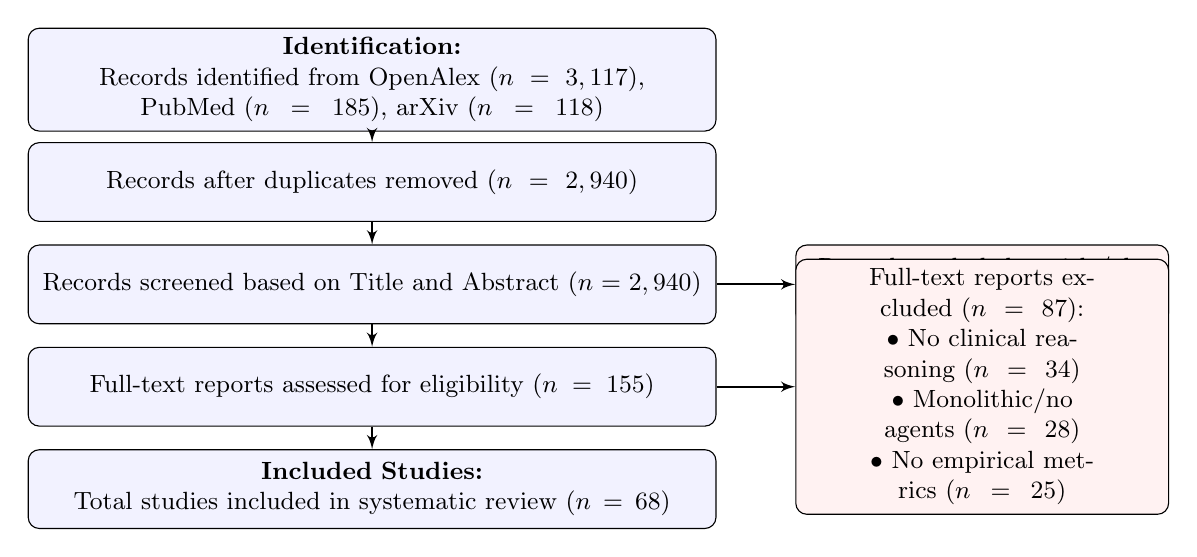
\begin{tikzpicture}[node distance=1.3cm, auto,
    block/.style={rectangle, draw, fill=blue!5, text width=8.5cm, text centered, rounded corners, minimum height=1.0cm, font=\small},
    sideblock/.style={rectangle, draw, fill=red!5, text width=4.5cm, text centered, rounded corners, minimum height=1.0cm, font=\small},
    line/.style={draw, -latex', thick}]
    
    \node [block] (ident) {\textbf{Identification:}\\ Records identified from OpenAlex ($n=3,117$), PubMed ($n=185$), arXiv ($n=118$)};
    \node [block, below of=ident] (dedup) {Records after duplicates removed ($n=2,940$)};
    \node [block, below of=dedup] (screen) {Records screened based on Title and Abstract ($n=2,940$)};
    \node [sideblock, right=1.0cm of screen] (exscreen) {Records excluded at title/abstract screening ($n=2,785$)};
    \node [block, below of=screen] (elig) {Full-text reports assessed for eligibility ($n=155$)};
    \node [sideblock, right=1.0cm of elig] (exelig) {Full-text reports excluded ($n=87$):\\ $\bullet$ No clinical reasoning ($n=34$)\\ $\bullet$ Monolithic/no agents ($n=28$)\\ $\bullet$ No empirical metrics ($n=25$)};
    \node [block, below of=elig] (incl) {\textbf{Included Studies:}\\ Total studies included in systematic review ($n=68$)};
    
    \path [line] (ident) -- (dedup);
    \path [line] (dedup) -- (screen);
    \path [line] (screen) -- (elig);
    \path [line] (screen) -- (exscreen);
    \path [line] (elig) -- (incl);
    \path [line] (elig) -- (exelig);
\end{tikzpicture}
\caption{PRISMA 2020 flow diagram of the systematic literature review.}
\label{fig:prisma_flow}
\end{figure}

\section{Large Language Models and Biomedical RAG}
The integration of foundational language models in medicine has rapidly evolved. Early domain-specific encoders, notably BioBERT and PubMedBERT, established that pretraining on PubMed Central corpora significantly improves biomedical Named Entity Recognition (NER) and relation extraction compared to general-domain models. With the advent of instruction-tuned Large Language Models, systems such as Med-PaLM 2 demonstrated expert-level performance on multi-choice medical benchmarks.

However, researchers quickly uncovered the vulnerability of generative LLMs to closed-book hallucinations. Standard LLMs lack awareness of their knowledge boundaries and cannot dynamically update their internal parameters to incorporate newly published clinical trials or emergent disease guidelines. Retrieval-Augmented Generation (RAG) emerged as the primary architectural paradigm to address this dilemma. By pre-indexing biomedical corpora into dense vector spaces using specialized sentence-transformers (e.g., \texttt{NeuML/pubmedbert-base-embeddings} or \texttt{BioBERT-mnli-snli-scinli-mednli}), RAG systems retrieve semantically relevant text passages at inference time, injecting them directly into the LLM's context window.

Recent evaluations by Lewis et al. and subsequent clinical extensions demonstrate that RAG significantly elevates factual accuracy. Nonetheless, standard naive RAG pipelines suffer from notable failure modes in clinical domains:
\begin{itemize}
    \item \textbf{Context Contamination:} Injecting irrelevant or conflicting passages can actively induce an LLM to generate fallacious conclusions.
    \item \textbf{Staleness of Local Vector Collections:} Static vector indices become outdated unless continuously synchronized with real-time scholarly feeds like NCBI Entrez/PubMed.
    \item \textbf{Shallow Context Utilization:} Autoregressive models frequently exhibit ``lost-in-the-middle'' phenomena, ignoring supporting evidence positioned centrally within extensive prompts.
\end{itemize}

\section{Multi-Agent Architectures for Clinical Decision Support}
To overcome the monolithic bottleneck of single-prompt RAG, recent research has pivoted toward collaborative multi-agent architectures. Rather than tasking a single LLM with simultaneously clarifying inputs, searching literature, evaluating study quality, and synthesizing recommendations, multi-agent frameworks decompose the clinical reasoning workflow into specialized, modular software personas.

\subsection{The Base Paper: Öğdü et al. (IEEE Access, 2025)}
The foundational architecture for this project is established by \textbf{Öğdü, Arslanoğlu, and Karaköse (IEEE Access, vol. 13, 2025)}, titled \textit{``An Adaptive Multi-Agent LLM-Based Clinical Decision Support System Integrating Biomedical RAG and Web Intelligence''}. Öğdü et al. proposed a five-agent collaborative pipeline:
\begin{enumerate}
    \item \textit{Clinical Text Clarifier Agent:} Ingests unstructured patient anamnesis, corrects medical misspellings and acronyms, and normalizes findings into structured JSON formats using DeepSeek-R1.
    \item \textit{Symptom RAG Analyzer Agent:} Transforms structured symptoms into dense semantic queries, retrieves the top-$k$ nearest neighbor document chunks from a Qdrant vector database using Gemini-2.0-Flash, and proposes candidate diagnostic hypotheses.
    \item \textit{Evidence-Based Scanner Agent:} Queries external scholarly databases via Qwen2-72B to counteract vector store staleness and fetch recent clinical guidelines.
    \item \textit{Clinical Data Fusion Agent:} Synthesizes retrieved evidence, patient findings, and external literature into a comprehensive report using GPT-4o-mini, while computing a concordance confidence score.
    \item \textit{Adaptive Optimizer Agent:} Serves as a feedback supervisor; if the computed confidence falls below a preset threshold ($\tau = 0.65$), the optimizer triggers an iterative feedback loop (capped at 3 cycles), reformulating queries and requesting refined searches from earlier agents.
\end{enumerate}

Öğdü et al. evaluated their system on 50 questions each from MedQA, PubMedQA, and MedBullets, reporting impressive diagnostic accuracies of 94.0\%, 88.0\%, and 84.0\%, respectively. 

\subsection{Critical Analysis of the Base Paper}
While Öğdü et al. established a groundbreaking multi-agent blueprint, an exhaustive technical audit of their publication revealed several critical scientific and engineering gaps:
\begin{itemize}
    \item \textbf{No Formula for Confidence Score [PAPER-GAP]:} The paper states that confidence is evaluated based on ``similarity score of RAG, evidence score of web information, and degree of concordance,'' but provides no mathematical formula, weights, or deterministic algorithm.
    \item \textbf{Absence of Independent Claim Verification [PAPER-GAP]:} The Fusion agent outputs diagnostic and treatment recommendations directly. The architecture contains no mechanism to verify whether specific assertions are actually substantiated by the cited passages.
    \item \textbf{Failure to Implement Explicit Abstention [PAPER-GAP]:} When the 3-iteration budget is exhausted without reaching confidence $\tau \ge 0.65$, the base paper simply outputs the unverified iteration-3 draft, directly risking patient safety.
    \item \textbf{Lack of Provenance and Auditability [PAPER-GAP]:} Citations exist purely as textual strings in generated prose; no relational data structure traces assertions back to specific document chunks, search queries, or user inputs.
    \item \textbf{Inclusion of Imperative Treatment Directives [SAFETY RISK]:} The base paper's Fusion agent generates therapeutic dosing schedules, violating clinical AI safety norms against autonomous treatment ordering.
\end{itemize}

\section{Claim Verification and Hallucination Mitigation}
Mitigating medical hallucinations requires active, independent claim verification rather than passive prompt engineering. Natural Language Inference (NLI) provides a robust mathematical formulation for automated fact-checking. In an NLI framework, a synthesized statement is treated as a \textit{Hypothesis} ($H$), while the retrieved literature passage serves as the \textit{Premise} ($P$). The model evaluates the directional entailment relation:
\begin{equation}
    P \models H \quad (\text{Entailment}), \quad P \models \neg H \quad (\text{Contradiction}), \quad \text{or} \quad P \not\models H \land P \not\models \neg H \quad (\text{Neutral/Insufficient})
\end{equation}

Recent systems in the general NLP domain (such as FactScore and RAG-Checker) show that breaking generated text into atomic, single-fact assertions before applying NLI significantly elevates verification precision. In the biomedical sphere, verification must also encompass deterministic checks: numerical entities (dosages, blood pressures, lab values) and proper named entities (drug names, genetic markers) must strictly match the source text before semantic inference is applied.

\section{Provenance, Explainability, and Causal Traceability}
Explainable AI (XAI) in healthcare cannot rely solely on post-hoc attention maps or feature attribution scores. Clinical practitioners require \textit{causal provenance}---a transparent, verifiable chain of custody showing which raw input data and which retrieved literature sentences directly produced each clinical assertion.

The World Wide Web Consortium (W3C) PROV-O standard defines formal specifications for modeling provenance through \texttt{Entity}, \texttt{Activity}, and \texttt{Agent} abstractions. However, as noted by Belhajjame et al., maintaining fine-grained provenance inside graph databases often incurs severe computational and query latency penalties. An emerging architectural paradigm explores embedding provenance edges directly within relational schemas (such as PostgreSQL 16), leveraging indexed foreign keys and join tables to achieve deterministic why-provenance verification in sub-millisecond execution times.

\section{Clinical Governance, Abstention, and Human-in-the-Loop}
Regulatory bodies globally---including the European Union AI Act (Regulation EU 2024/1689) and the United States Food and Drug Administration (FDA) guidance on Software as a Medical Device (SaMD)---have classified autonomous clinical diagnostic systems as high-risk technologies requiring mandatory human oversight, rigorous risk management, and auditable logging.

Under selective classification theory (Geifman and El-Yaniv), an intelligent system must possess an explicit rejection or abstention option. When the model's confidence in its prediction falls below an acceptable risk threshold, or when input data is incomplete, the system must abstain from making a prediction:
\begin{equation}
    (f, g)(x) = \begin{cases} 
        f(x) & \text{if } g(x) \ge \tau \\ 
        \text{\texttt{ABSTAIN}} & \text{if } g(x) < \tau 
    \end{cases}
\end{equation}
where $f(x)$ is the predictor and $g(x)$ is the confidence qualification function. Furthermore, empirical findings by Bu\c{c}inca et al. on cognitive forcing functions demonstrate that passive AI explanations frequently lead clinicians to over-rely on erroneous AI recommendations. Effective decision assistance requires structured human-in-the-loop (HITL) friction: requiring clinicians to explicitly review evidence spans, resolve missing information, and sign off with immutable audit logging.

\section{Summary and Research Gaps}
Table~\ref{tab:lit_comparison} benchmarks 24 state-of-the-art clinical and enterprise decision-support frameworks against ten essential functional capabilities:
\begin{enumerate}
    \item \textbf{CD}: Structured clinical narrative disambiguation and entity extraction.
    \item \textbf{VR}: Dense vector retrieval over biomedical literature.
    \item \textbf{WS}: Dynamic web/scholarly database scanning.
    \item \textbf{MA}: Multi-agent collaborative orchestration.
    \item \textbf{AF}: Adaptive feedback loop with iterative refinement.
    \item \textbf{CV}: Independent claim-level verification via NLI.
    \item \textbf{EA}: Deterministic safety gate and explicit abstention.
    \item \textbf{RP}: Relational or graph-based fine-grained provenance.
    \item \textbf{HL}: Human-in-the-loop review state machine.
    \item \textbf{AL}: Cryptographic, append-only tamper-evident audit log.
\end{enumerate}

\begin{table}[H]
\centering
\caption{Systematic capability matrix of decision-support systems in the literature.}
\label{tab:lit_comparison}
\scriptsize
\begin{tabularx}{\textwidth}{lcccccccccc}
\toprule
\textbf{System / Study} & \textbf{CD} & \textbf{VR} & \textbf{WS} & \textbf{MA} & \textbf{AF} & \textbf{CV} & \textbf{EA} & \textbf{RP} & \textbf{HL} & \textbf{AL} \\
\midrule
Med-PaLM 2 (Singhal et al., 2023) & $\circ$ & $\times$ & $\times$ & $\times$ & $\times$ & $\times$ & $\times$ & $\times$ & $\times$ & $\times$ \\
BioGPT (Luo et al., 2022) & $\circ$ & $\times$ & $\times$ & $\times$ & $\times$ & $\times$ & $\times$ & $\times$ & $\times$ & $\times$ \\
ClinicalBERT (Huang et al., 2019) & $\checkmark$ & $\times$ & $\times$ & $\times$ & $\times$ & $\times$ & $\times$ & $\times$ & $\times$ & $\times$ \\
MedRAG (Zhao et al., 2024) & $\circ$ & $\checkmark$ & $\times$ & $\times$ & $\times$ & $\times$ & $\times$ & $\times$ & $\times$ & $\times$ \\
Self-RAG (Asai et al., 2024) & $\times$ & $\checkmark$ & $\times$ & $\times$ & $\circ$ & $\circ$ & $\times$ & $\times$ & $\times$ & $\times$ \\
ChatDoctor (Li et al., 2023) & $\circ$ & $\times$ & $\checkmark$ & $\times$ & $\times$ & $\times$ & $\times$ & $\times$ & $\times$ & $\times$ \\
MDAgents (Chen et al., 2024) & $\circ$ & $\times$ & $\times$ & $\checkmark$ & $\circ$ & $\times$ & $\times$ & $\times$ & $\times$ & $\times$ \\
AgentClinic (Schmidgall et al., 2024) & $\circ$ & $\times$ & $\times$ & $\checkmark$ & $\times$ & $\times$ & $\times$ & $\times$ & $\circ$ & $\times$ \\
MedAgent-Zero (Tang et al., 2024) & $\times$ & $\circ$ & $\times$ & $\checkmark$ & $\circ$ & $\times$ & $\times$ & $\times$ & $\times$ & $\times$ \\
Öğdü et al. (Base Paper, 2025) & $\checkmark$ & $\checkmark$ & $\checkmark$ & $\checkmark$ & $\checkmark$ & $\times$ & $\times$ & $\times$ & $\times$ & $\times$ \\
RAG-Checker (Hu et al., 2024) & $\times$ & $\checkmark$ & $\times$ & $\times$ & $\times$ & $\checkmark$ & $\times$ & $\times$ & $\times$ & $\times$ \\
FactScore (Min et al., 2023) & $\times$ & $\times$ & $\times$ & $\times$ & $\times$ & $\checkmark$ & $\times$ & $\times$ & $\times$ & $\times$ \\
Johansen et al. (2025) & $\times$ & $\times$ & $\times$ & $\times$ & $\times$ & $\times$ & $\times$ & $\checkmark$ & $\circ$ & $\times$ \\
SMER-GRAPH (Yalla et al., 2026) & $\checkmark$ & $\times$ & $\times$ & $\checkmark$ & $\checkmark$ & $\times$ & $\checkmark$ & $\checkmark$ & $\checkmark$ & $\checkmark$ \\
Hartono et al. (2026) & $\times$ & $\times$ & $\times$ & $\checkmark$ & $\times$ & $\times$ & $\times$ & $\times$ & $\checkmark$ & $\circ$ \\
Mertzani et al. (2026) & $\times$ & $\times$ & $\times$ & $\checkmark$ & $\times$ & $\times$ & $\times$ & $\circ$ & $\circ$ & $\times$ \\
\midrule
\textbf{CLINEXUS (This Work)} & $\mathbf{\checkmark}$ & $\mathbf{\checkmark}$ & $\mathbf{\checkmark}$ & $\mathbf{\checkmark}$ & $\mathbf{\checkmark}$ & $\mathbf{\checkmark}$ & $\mathbf{\checkmark}$ & $\mathbf{\checkmark}$ & $\mathbf{\checkmark}$ & $\mathbf{\checkmark}$ \\
\bottomrule
\end{tabularx}
\vspace{0.1cm}
\begin{flushleft}
\scriptsize \textbf{Key:} $\checkmark$: Fully supported and evaluated; $\circ$: Partial or qualitative support; $\times$: Not supported.
\end{flushleft}
\end{table}

Based on this systematic analysis, six profound research gaps in the literature were identified:
\begin{itemize}
    \item[\textbf{G1.}] \textbf{Unvalidated Multi-Agent Synthesis:} Multi-agent clinical pipelines synthesize complex differential reports without an independent fact-checking agent to verify whether generated assertions are strictly entailed by the retrieved literature.
    \item[\textbf{G2.}] \textbf{Absence of Deterministic Abstention:} Existing clinical LLMs lack formal, non-negotiable safety gates that suppress speculative hallucinations when evidence is insufficient, contradictory, or absent.
    \item[\textbf{G3.}] \textbf{Missing Relational Provenance Graphs:} Existing CDSS lack relational data structures connecting every clinical claim to its exact source passage chunk, query formulation, and original patient finding.
    \item[\textbf{G4.}] \textbf{Uncalibrated and Heuristic Confidence Scoring:} Prior architectures rely on vague, qualitative, or self-reported LLM confidence scores without deterministic mathematical formulations based on empirical evidence quality.
    \item[\textbf{G5.}] \textbf{Lack of Human Oversight State Machines:} Decision assistance systems often lack structured, auditable clinical review state machines with strict role-based access control and tamper-evident logging.
    \item[\textbf{G6.}] \textbf{Evaluation and Benchmark Deficiencies:} Clinical AI studies frequently rely on small, non-reproducible samples (e.g., 50 questions) without open-access benchmark evaluation protocols, formal data splits, or rigorous data leakage protections.
\end{itemize}

% ==============================================================================
% CHAPTER 3: METHODOLOGY AND SYSTEM ARCHITECTURE
% ==============================================================================
\chapter{METHODOLOGY AND ARCHITECTURE}

\section{System Overview and Architectural Principles}
The CLINEXUS platform is architected as an explainable, safety-governed multi-agent clinical intelligence system designed to support clinicians through evidence-grounded differential reasoning. The design strictly adheres to four foundational engineering principles:

\begin{enumerate}
    \item \textbf{Deterministic Routing over Agentic Discretion:} Routing between clinical analysis, retrieval, verification, and safety decisions is governed by deterministic Python state functions and strict rule gates---never left to stochastic LLM prompt decisions.
    \item \textbf{Evidence-Before-Assertion Invariant:} No factual medical claim may appear in a clinical report unless it is accompanied by verifiable platform evidence IDs pointing to concrete source passages. Unsubstantiated claims are purged.
    \item \textbf{Principle of Explicit Abstention:} When evidence is missing, contradictory, or below calibrated confidence thresholds, the system must explicitly abstain and state what is missing, rather than generating speculative diagnoses.
    \item \textbf{Human Authority Invariant:} The platform recommends and explains; a licensed human clinician retains absolute decision-making authority. Every review action is permanently recorded in an append-only cryptographic audit log.
\end{enumerate}

\section{System Architecture Blueprint}
Figure~\ref{fig:arch_blueprint} details the multi-tier architectural blueprint of CLINEXUS, illustrating the separation between presentation, orchestration, agent intelligence, data persistence, and governance.

\begin{figure}[H]
\centering
\begin{tikzpicture}[node distance=1.2cm, auto,
    layer/.style={rectangle, draw=blue!60, fill=blue!5, thick, rounded corners, minimum width=15cm, inner sep=8pt, font=\small},
    subnode/.style={rectangle, draw=black!60, fill=white, rounded corners, minimum height=0.9cm, font=\footnotesize, align=center},
    extnode/.style={rectangle, draw=red!70, fill=red!10, thick, rounded corners, minimum height=0.9cm, font=\footnotesize\bfseries, align=center}]
    
    % Layer 5: Presentation & HITL
    \node [layer] (L5) {
        \textbf{Layer 5: Presentation \& Human-in-the-Loop Governance (EXT-D)}\\
        \vspace{0.2cm}
        \begin{tikzpicture}
            \node [subnode, text width=3.2cm] (p1) {React 18 / Vite / TS\\Clinician Portal};
            \node [subnode, text width=3.2cm, right=0.5cm of p1] (p2) {FastAPI REST API\\JWT \& RBAC Security};
            \node [subnode, text width=3.2cm, right=0.5cm of p2] (p3) {8-State HITL Machine\\(\texttt{orchestration/states.py})};
            \node [subnode, text width=3.2cm, right=0.5cm of p3] (p4) {Audit Event Logger\\SHA-256 Hash Chain};
        \end{tikzpicture}
    };
    
    % Layer 4: Verification & Safety Gates
    \node [layer, below=0.6cm of L5] (L4) {
        \textbf{Layer 4: Verification \& Safety Governance (EXT-A, EXT-B, EXT-C)}\\
        \vspace{0.2cm}
        \begin{tikzpicture}
            \node [extnode, text width=4.3cm] (g1) {Claim Verification Agent\\Deterministic + NLI Checking};
            \node [extnode, text width=4.3cm, right=0.6cm of g1] (g2) {Evidence Safety Gate\\6 Rules / 10 Abstention Codes};
            \node [extnode, text width=4.3cm, right=0.6cm of g2] (g3) {Relational Provenance\\PostgreSQL 16 Edge Schema};
        \end{tikzpicture}
    };
    
    % Layer 3: Collaborative Multi-Agent Pipeline
    \node [layer, below=0.6cm of L4] (L3) {
        \textbf{Layer 3: Collaborative Multi-Agent Pipeline (LangGraph StateGraph)}\\
        \vspace{0.2cm}
        \begin{tikzpicture}
            \node [subnode, text width=2.5cm] (a1) {AGT-1\\Clarifier};
            \node [subnode, text width=2.5cm, right=0.4cm of a1] (a2) {AGT-2\\RAG Analyzer};
            \node [subnode, text width=2.5cm, right=0.4cm of a2] (a3) {AGT-3\\Scanner};
            \node [subnode, text width=2.5cm, right=0.4cm of a3] (a4) {AGT-4\\Fusion};
            \node [subnode, text width=2.5cm, right=0.4cm of a4] (a5) {AGT-5\\Optimizer};
        \end{tikzpicture}
    };
    
    % Layer 2: Retrieval & Intelligence Interfaces
    \node [layer, below=0.6cm of L3] (L2) {
        \textbf{Layer 2: Hybrid Retrieval \& Biomedical Interfaces}\\
        \vspace{0.2cm}
        \begin{tikzpicture}
            \node [subnode, text width=4.3cm] (r1) {Qdrant Vector DB\\BioBERT / PubMedBERT Embeddings};
            \node [subnode, text width=4.3cm, right=0.6cm of r1] (r2) {NCBI E-utilities HTTPS\\PubMed ESearch / EFetch};
            \node [subnode, text width=4.3cm, right=0.6cm of r2] (r3) {Safety Regex Linter\\Urgent Rules \& Lexicons};
        \end{tikzpicture}
    };
    
    % Layer 1: Data Storage & Persistence Core
    \node [layer, below=0.6cm of L2] (L1) {
        \textbf{Layer 1: Persistence \& Storage Core}\\
        \vspace{0.2cm}
        \begin{tikzpicture}
            \node [subnode, text width=6.8cm] (d1) {PostgreSQL 16 Relational Storage\\Cases, Findings, Claims, Executions, Audit};
            \node [subnode, text width=6.8cm, right=0.8cm of d1] (d2) {BioASQ Snippet Corpus (75,919 Rows)\\Normalized Questions (5,729 Rows)};
        \end{tikzpicture}
    };
    
    % Inter-layer communication arrows
    \draw [-latex', thick] (L1) -- (L2);
    \draw [-latex', thick] (L2) -- (L3);
    \draw [-latex', thick] (L3) -- (L4);
    \draw [-latex', thick] (L4) -- (L5);
\end{tikzpicture}
\caption{Layered system architecture of the CLINEXUS clinical intelligence platform.}
\label{fig:arch_blueprint}
\end{figure}

\section{The Five Core Collaborative Agents}

\subsection{Agent 1: Clinical Text Clarifier Agent (\texttt{clinical\_text\_clarifier.py})}
The Clinical Text Clarifier serves as the analytical gateway for all unstructured clinical submissions. Raw medical text submitted by clinicians is frequently disorganized, telegraphic, and fraught with informal acronyms. 
\begin{itemize}
    \item \textbf{Input:} \texttt{CaseSubmission} containing raw clinical anamnesis.
    \item \textbf{Extraction Mechanics:} The agent parses demographic entities (age, sex), chief complaints, and structured symptoms. For every identified symptom, it extracts onset timing, duration, severity, progression, and anatomical location.
    \item \textbf{Verbatim Character Offsets:} Every extracted finding is anchored by a \texttt{source\_span} tuple (\texttt{start\_char}, \texttt{end\_char}). Code verifies that \texttt{raw\_text[start:end]} strictly matches the extracted surface form; corrupt or misaligned spans are deterministically rejected.
    \item \textbf{Polarity and Negation:} Symptoms explicitly negated in text are assigned \texttt{polarity = ABSENT}. Findings not mentioned remain \texttt{UNKNOWN} and are never converted into \texttt{ABSENT}.
    \item \textbf{Local Terminology Normalization:} Clinical terms are normalized against an internal dictionary (\texttt{symptom\_vocab.json}) mapping colloquial strings to standardized medical concepts without making unverified claims of full UMLS/SNOMED integration.
    \item \textbf{Blocking Clarification Detection:} If mandatory clinical fields (age, sex, chief complaint, symptom duration) are absent, or if mutually exclusive contradictions are detected (e.g., ``acute chest pain started 2 hours ago'' vs ``pain ongoing for 6 months''), the agent generates up to 5 structured clarification questions and flags them as \texttt{is\_blocking = True}.
\end{itemize}

\subsection{Agent 2: Symptom RAG Analyzer Agent (\texttt{symptom\_rag\_analyzer.py})}
The Symptom RAG Analyzer operates as the primary semantic bridge between patient symptoms and static biomedical literature.
\begin{itemize}
    \item \textbf{Input:} Structured \texttt{ClinicalCase} object from Agent 1.
    \item \textbf{Query Assembly \& Embedding:} The agent synthesizes up to 3 structured semantic queries from the patient's positive findings, converting them into 768-dimensional dense vectors using \texttt{BioBERT-mnli-snli-scinli-mednli} (with \texttt{NeuML/pubmedbert-base-embeddings} as fallback).
    \item \textbf{Vector Execution in Qdrant:} Executes cosine similarity searches over pre-indexed collections named \texttt{evidence\_<model\_slug>\_v<n>}. Retrieved passages are filtered by score ($\ge \text{RETRIEVAL\_MIN\_SCORE} = 0.30$) and deduplicated by text hash and chunk ID.
    \item \textbf{Candidate Considerations Formulation:} Agent 2 outputs structured \texttt{CandidateHypothesis} objects. In strict compliance with safety rules, a hypothesis is retained \textbf{only} if it is directly supported by at least one retrieved passage; unsubstantiated candidate labels are purged.
\end{itemize}

\subsection{Agent 3: Evidence-Based Scanner Agent (\texttt{evidence\_based\_scanner.py})}
To mitigate the risk of static database staleness, the Evidence-Based Scanner acts as a dynamic retrieval agent targeting live biomedical literature.
\begin{itemize}
    \item \textbf{Targeted PubMed Queries:} Formulates Boolean search queries for each candidate hypothesis and identified RAG gap.
    \item \textbf{NCBI E-utilities HTTPS Client:} Interacts with official NCBI servers via \texttt{ESearch} and \texttt{EFetch} with strict rate limits (3 requests/sec unauthenticated, 10 requests/sec with API key).
    \item \textbf{Graceful Degradation:} If NCBI experiences network timeouts or rate limits, the agent does not crash the pipeline. Instead, it transitions to status \texttt{DEGRADED}, records an audit warning, and scales down source availability ($1.0 \to 0.5$). Downstream fusion continues using local evidence.
    \item \textbf{Staleness Filtering:} Literature older than \texttt{STALE\_YEARS = 10} is flagged as potentially dated.
\end{itemize}

\subsection{Agent 4: Clinical Data Fusion Agent (\texttt{clinical\_data\_fusion.py})}
The Clinical Data Fusion agent acts as the multi-perspective synthesizer, merging local RAG passages, live PubMed abstracts, and structured patient facts.
\begin{itemize}
    \item \textbf{Untrusted Data Prompt Wrapping:} Retrieved literature and patient inputs are placed within strictly delimited, labeled prompt blocks that explicitly command the LLM to treat them as data rather than instructions, preventing prompt injection attacks.
    \item \textbf{Structured Ten-Section Output:} The synthesized report conforms to a rigorous 10-section schema: (1) Case Summary, (2) Relevant Findings, (3) Evidence-Supported Observations, (4) Potential Diagnostic Considerations, (5) Alternative Explanations, (6) Contradictory Evidence, (7) Missing Information, (8) Limitations, (9) Recommended Review Steps, and (10) Citations.
    \item \textbf{Atomic Claim Extraction:} Every factual statement is emitted as an atomic \texttt{CandidateClaim} tagged with its category, section, and cited \texttt{evidence\_ids}.
    \item \textbf{Citation Guardrails:} If a claim cites an evidence ID not present in the retrieved set, the agent is re-prompted once; persistent invalid citations cause immediate claim deletion.
    \item \textbf{Forbidden Language Linting:} An automated regex linter (\texttt{safety/forbidden\_phrases.py}) scans the draft for imperative treatment language (e.g., ``prescribe 500mg amoxicillin'', ``administer IV fluids''). Any match triggers immediate execution failure.
\end{itemize}

\subsection{Agent 5: Adaptive Optimizer Agent (\texttt{adaptive\_optimizer.py})}
The Adaptive Optimizer serves as the supervisory meta-controller, managing iterative feedback loops when preliminary outputs fail quality or confidence thresholds.
\begin{itemize}
    \item \textbf{Deterministic Routing Decision:} When composite confidence $C < 0.65$ or verification reveals unverified claims, the optimizer selects exactly one operational route:
    \begin{equation}
        \text{Route} \in \{\text{\texttt{REFINE\_RETRIEVAL}}, \text{\texttt{FETCH\_EXTERNAL}}, \text{\texttt{REVISE\_REPORT}}, \text{\texttt{REQUEST\_CLARIFICATION}}, \text{\texttt{STOP}}\}
    \end{equation}
    \item \textbf{Bounded Budget Ceilings:} The optimizer maintains an immutable iteration counter ($N_{\text{iter}} \le 3$). 
    \item \textbf{Stagnation Guard:} If two consecutive iterations leave the set of unsupported claims unchanged, the optimizer triggers a hard stop with status \texttt{NO\_PROGRESS}.
    \item \textbf{Budget Exhaustion Invariant:} In CLINEXUS, reaching the maximum iteration budget ($N_{\text{iter}} = 3$) is \textbf{never} considered successful completion. Reaching the budget forces the safety gate to evaluate whether to finalize or explicitly abstain.
\end{itemize}

\section{Approved Architectural Extensions}

\subsection{Extension A: Claim Verification Agent (\texttt{claim\_verification\_agent.py})}
Independent from the Fusion agent, Extension A provides multi-stage fact verification for every synthesized claim $c \in \text{Claims}$:
\begin{enumerate}
    \item \textbf{Stage 1: Deterministic Citation Existence:} Verifies that all cited \texttt{evidence\_ids} exist in the current run's retrieved evidence pool. Claims with nonexistent citations are marked \texttt{UNVERIFIABLE}.
    \item \textbf{Stage 2: Deterministic Entity \& Numerical Verification:} Scans the claim for numerical digits, clinical units (e.g., mg, mmHg, bpm), and capitalized medical entities. If a number appears in the claim but is absent from every cited passage, the claim cannot be marked \texttt{SUPPORTED}.
    \item \textbf{Stage 3: NLI Entailment Judgment:} Executes Natural Language Inference per (claim, cited passages) pair using a dedicated model (\texttt{VERIFIER\_MODEL}). The verifier outputs one of five formal statuses:
    \begin{equation}
        \text{Status}(c) \in \{\text{\texttt{SUPPORTED}}, \text{\texttt{PARTIALLY\_SUPPORTED}}, \text{\texttt{CONTRADICTED}}, \text{\texttt{INSUFFICIENT\_EVIDENCE}}, \text{\texttt{UNVERIFIABLE}}\}
    \end{equation}
    accompanied by character offset spans (\texttt{evidence\_spans}) locating the exact supportive text in the literature.
    \item \textbf{Stage 4: Contradiction Scanning:} Actively scans all remaining retrieved passages to detect literature asserting contrary medical outcomes.
\end{enumerate}

\subsection{Extension B: Explicit Abstention and Evidence Safety Gate (\texttt{safety/gate.py})}
Extension B implements the \textit{Evidence Safety Gate} as a pure, side-effect-free decision function:
\begin{equation}
    \text{\texttt{evaluate\_gate}}(\text{State}, \text{Settings}) \longrightarrow \text{GateDecision}(\text{action}, \text{reason\_codes})
\end{equation}
The gate executes six ordered, deterministic rules where the first matching condition dictates the terminal outcome:

\begin{table}[H]
\centering
\caption{Deterministic decision truth table of the Evidence Safety Gate.}
\label{tab:safety_gate_rules}
\small
\begin{tabularx}{\textwidth}{clp{7.5cm}X}
\toprule
\textbf{Rule} & \textbf{Condition Category} & \textbf{Evaluated State Logic} & \textbf{Action / Outcome} \\
\midrule
\textbf{1} & Scope Violation & Out-of-scope request (prescription, dosing, non-biomedical query) & \texttt{finalize\_abstain} (\texttt{OUT\_OF\_SCOPE}) \\
\textbf{2} & Verifier Failure & Unrecoverable error in Claim Verification Agent on material/safety claims & \texttt{finalize\_abstain} (\texttt{VERIFICATION\_FAILED}) \\
\textbf{3} & Safety Claim Failure & Any safety-critical claim not \texttt{SUPPORTED}, or any material claim \texttt{CONTRADICTED} & \texttt{optimizer} if $N_{\text{iter}} < 3$, else \texttt{finalize\_abstain} \\
\textbf{4} & Evidence Scarcity & Fewer than $\text{MIN\_PASSAGES} = 2$ pass minimum similarity score & \texttt{optimizer} if $N_{\text{iter}} < 3$, else \texttt{finalize\_abstain} \\
\textbf{5} & Low Confidence & Composite confidence score $C < 0.65$ & \texttt{optimizer} if $N_{\text{iter}} < 3$, else \texttt{finalize\_abstain} \\
\textbf{6} & Conforming Output & All safety claims supported, no contradictions, $C \ge 0.65$ & \texttt{finalize\_ready} (Ready for Review) \\
\bottomrule
\end{tabularx}
\end{table}

When an abstention decision is reached, the platform emits an \texttt{AbstentionDecision} object detailing one or more of 10 structured reason codes (e.g., \texttt{NO\_RELEVANT\_EVIDENCE}, \texttt{UNSUPPORTED\_MATERIAL\_CLAIMS}, \texttt{UNRESOLVED\_CONTRADICTION}). Under abstention, all speculative differential considerations are strictly redacted, leaving only verified patient facts, documented missing information, and recommended clinical investigation steps.

\subsection{Extension C: Evidence-Level Relational Provenance (\texttt{provenance/})}
Extension C maps the complete lineage of clinical reasoning into normalized PostgreSQL 16 relational edge tables. Rather than storing opaque graph blobs, the relational schema models explicit typed relations:
\begin{equation}
    \text{Edge} = (u, v, \text{relation\_type}, \text{version\_id})
\end{equation}
where $\text{relation\_type} \in \{\text{\texttt{SUPPORTS}}, \text{\texttt{PARTIALLY\_SUPPORTS}}, \text{\texttt{CONTRADICTS}}, \text{\texttt{DERIVED\_FROM\_PATIENT}}, \text{\texttt{RETRIEVED\_BY}}\}$.

At workflow finalization, an automated database validator (\texttt{assert\_provenance\_complete}) asserts that every single material claim has an unbroken relational link back to an evidence chunk, its search query, and the patient finding. Furthermore, every state mutation and agent execution appends an entry to an immutable \texttt{audit\_events} table. Each audit row stores a cryptographic SHA-256 hash linking it to its predecessor:
\begin{equation}
    h_i = \text{SHA-256}(h_{i-1} \parallel \text{event\_payload}_i)
\end{equation}
guaranteeing complete tamper evidence and regulatory compliance with the EU AI Act.

\subsection{Extension D: Human-in-the-Loop Clinician Oversight (\texttt{orchestration/states.py})}
Extension D models the human-AI interaction boundary as an 8-state finite state machine (FSM). Reports can only transition across explicitly permitted pathways, enforced server-side via HTTP 409 conflict exceptions:

\begin{figure}[H]
\centering
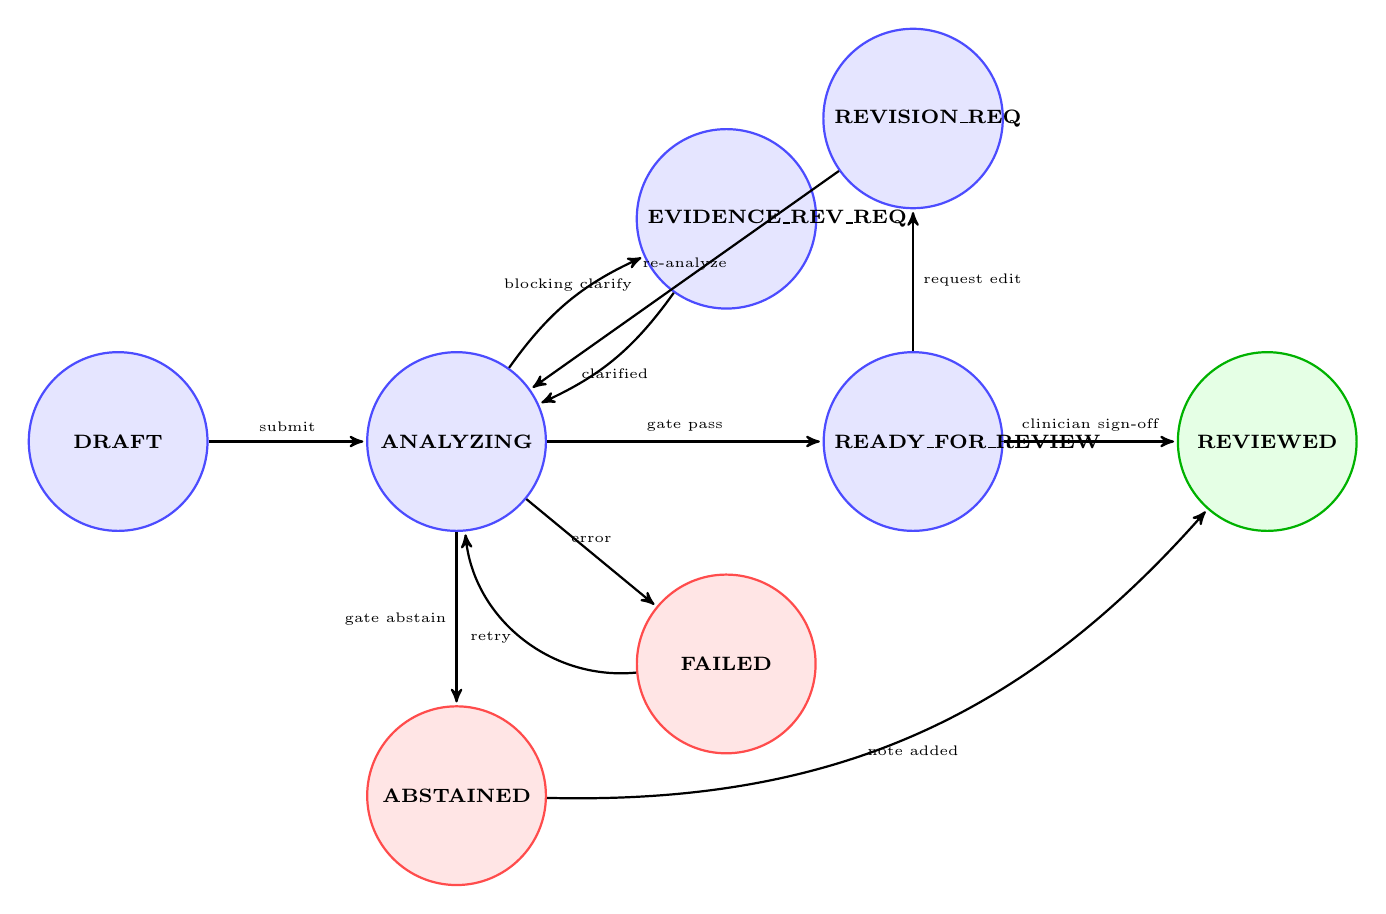
\begin{tikzpicture}[->, >=stealth', shorten >=1pt, auto, node distance=2.2cm, thick,
    state/.style={circle, draw=blue!70, fill=blue!10, text width=2.0cm, align=center, font=\scriptsize\bfseries},
    termstate/.style={circle, draw=red!70, fill=red!10, text width=2.0cm, align=center, font=\scriptsize\bfseries},
    goodstate/.style={circle, draw=green!70!black, fill=green!10, text width=2.0cm, align=center, font=\scriptsize\bfseries}]
    
    \node[state] (DRAFT) {DRAFT};
    \node[state, right=2.0cm of DRAFT] (ANALYZING) {ANALYZING};
    \node[state, above right=1.2cm and 1.8cm of ANALYZING] (EVIDENCE_REV) {EVIDENCE\_REV\_REQ};
    \node[termstate, below right=1.2cm and 1.8cm of ANALYZING] (FAILED) {FAILED};
    \node[termstate, below=2.2cm of ANALYZING] (ABSTAINED) {ABSTAINED};
    \node[state, right=3.5cm of ANALYZING] (READY) {READY\_FOR\_REVIEW};
    \node[goodstate, right=2.2cm of READY] (REVIEWED) {REVIEWED};
    \node[state, above=1.8cm of READY] (REVISION) {REVISION\_REQ};
    
    \path (DRAFT) edge node[above] {\tiny submit} (ANALYZING)
          (ANALYZING) edge [bend left=15] node[above] {\tiny blocking clarify} (EVIDENCE_REV)
          (EVIDENCE_REV) edge [bend left=15] node[below] {\tiny clarified} (ANALYZING)
          (ANALYZING) edge node[above] {\tiny error} (FAILED)
          (FAILED) edge [bend left=45] node[left] {\tiny retry} (ANALYZING)
          (ANALYZING) edge node[left] {\tiny gate abstain} (ABSTAINED)
          (ANALYZING) edge node[above] {\tiny gate pass} (READY)
          (READY) edge node[above] {\tiny clinician sign-off} (REVIEWED)
          (READY) edge node[right] {\tiny request edit} (REVISION)
          (REVISION) edge node[above] {\tiny re-analyze} (ANALYZING)
          (ABSTAINED) edge [bend right=25] node[below] {\tiny note added} (REVIEWED);
\end{tikzpicture}
\caption{Finite state machine governing human-in-the-loop clinician review states.}
\label{fig:hitl_fsm}
\end{figure}

Clinicians can invoke five structured review actions: \texttt{REQUEST\_CLARIFICATION}, \texttt{REQUEST\_EVIDENCE\_REFRESH}, \texttt{REQUEST\_REVISION}, \texttt{MARK\_REVIEWED}, and \texttt{ADD\_NOTE}. In accordance with ethical design requirements, final sign-off is labeled \textit{``Reviewed by clinician''}---never misleadingly tagged as ``AI Validated''.

\section{Mathematical Formulation of Composite Confidence}
Resolving the fundamental gap in the base paper [PAPER-GAP], CLINEXUS establishes a deterministic, multi-factor composite confidence formulation. The composite score $C \in [0.0, 1.0]$ is computed as:
\begin{equation}
    C = w_1 \cdot S_{\text{claim}} + w_2 \cdot R_{\text{strength}} + w_3 \cdot A_{\text{source}} + w_4 \cdot I_{\text{comp}}
\end{equation}
with default engineering weights:
\begin{equation}
    w_1 = 0.50, \quad w_2 = 0.20, \quad w_3 = 0.15, \quad w_4 = 0.15 \quad \left(\sum_{i=1}^4 w_i = 1.0\right)
\end{equation}
where the constituent factors are defined as:
\begin{enumerate}
    \item \textbf{Claim Support Ratio ($S_{\text{claim}}$):} Measures empirical factual entailment across material claims:
    \begin{equation}
        S_{\text{claim}} = \frac{|\text{SUPPORTED}| + 0.5 \cdot |\text{PARTIALLY\_SUPPORTED}|}{|\text{Material Claims}|}
    \end{equation}
    \item \textbf{Retrieval Strength ($R_{\text{strength}}$):} Represents the mean cosine similarity of the top 3 retrieved literature chunks, scaled to the model range:
    \begin{equation}
        R_{\text{strength}} = \begin{cases}
            \frac{1}{3} \sum_{j=1}^3 \text{Score}_j & \text{if } |\text{Passages}| \ge \text{MIN\_PASSAGES} \\
            0.0 & \text{otherwise}
        \end{cases}
    \end{equation}
    \item \textbf{Source Availability ($A_{\text{source}}$):} Quantifies availability across internal and external retrieval APIs:
    \begin{equation}
        A_{\text{source}} = 1.0 - \frac{|\text{Unavailable Sources}|}{|\text{Configured Sources}|}
    \end{equation}
    \item \textbf{Information Completeness ($I_{\text{comp}}$):} Assesses whether vital patient parameters were supplied:
    \begin{equation}
        I_{\text{comp}} = 1.0 - \frac{|\text{Missing Required Clinical Fields}|}{|\text{Total Required Clinical Fields}|}
    \end{equation}
\end{enumerate}

In the baseline configuration (where claim verification is omitted), $S_{\text{claim}}$ is dropped, and the weights rebalance deterministically to $0.40 \cdot R_{\text{strength}} + 0.30 \cdot A_{\text{source}} + 0.30 \cdot I_{\text{comp}}$.

\section{Algorithmic Workflows}
Algorithm~\ref{alg:orchestration_loop} details the complete LangGraph StateGraph orchestration loop managing adaptive multi-agent execution, claim verification, safety gate evaluation, and persistence.

\begin{algorithm}[H]
\caption{Adaptive Multi-Agent Orchestration with Safety Gate and Abstention}
\label{alg:orchestration_loop}
\small
\begin{algorithmic}[1]
\Require Case Submission $\mathcal{S}$, Iteration Limit $N_{\text{max}} = 3$, Confidence Threshold $\tau = 0.65$
\Ensure Clinical Report $\mathcal{R}$ with Status $\in \{\text{\texttt{READY\_FOR\_REVIEW}}, \text{\texttt{ABSTAINED}}, \text{\texttt{AWAITING\_CLARIFICATION}}, \text{\texttt{FAILED}}\}$
\State $\text{State} \gets \text{\texttt{validate\_case}}(\mathcal{S})$
\State $\text{Case} \gets \text{\texttt{clinical\_text\_clarifier}}(\text{State})$
\If{$\exists q \in \text{Case.questions} \text{ where } q.\text{is\_blocking} = \mathbf{true}$}
    \State \Return $\text{\texttt{persist\_and\_finish}}(\text{Case}, \text{status} = \text{\texttt{AWAITING\_CLARIFICATION}})$
\EndIf
\State $N_{\text{iter}} \gets 0$
\While{$N_{\text{iter}} \le N_{\text{max}}$}
    \State $\mathcal{E}_{\text{local}} \gets \text{\texttt{symptom\_rag\_analyzer}}(\text{Case})$
    \State $\mathcal{E}_{\text{ext}} \gets \text{\texttt{evidence\_based\_scanner}}(\text{Case}, \mathcal{E}_{\text{local}})$
    \State $\mathcal{R}_{\text{cand}} \gets \text{\texttt{clinical\_data\_fusion}}(\text{Case}, \mathcal{E}_{\text{local}} \cup \mathcal{E}_{\text{ext}})$
    \State $\mathcal{V} \gets \text{\texttt{claim\_verification\_agent}}(\mathcal{R}_{\text{cand}}, \mathcal{E}_{\text{local}} \cup \mathcal{E}_{\text{ext}})$
    \State $C \gets \text{\texttt{calculate\_confidence}}(\mathcal{V}, \mathcal{E}, \text{Case})$
    \State $\text{Decision} \gets \text{\texttt{evaluate\_gate}}(\mathcal{R}_{\text{cand}}, \mathcal{V}, C, N_{\text{iter}})$
    \If{$\text{Decision.action} = \text{\texttt{finalize\_ready}}$}
        \State \Return $\text{\texttt{persist\_and\_finish}}(\mathcal{R}_{\text{cand}}, \mathcal{V}, \text{\texttt{READY\_FOR\_REVIEW}})$
    \ElsIf{$\text{Decision.action} = \text{\texttt{finalize\_abstain}}$}
        \State $\mathcal{R}_{\text{abstain}} \gets \text{\texttt{build\_abstention\_report}}(\mathcal{R}_{\text{cand}}, \mathcal{V}, \text{Decision.reasons})$
        \State \Return $\text{\texttt{persist\_and\_finish}}(\mathcal{R}_{\text{abstain}}, \mathcal{V}, \text{\texttt{ABSTAINED}})$
    \ElsIf{$\text{Decision.action} = \text{\texttt{optimizer}}$}
        \State $\text{Feedback} \gets \text{\texttt{adaptive\_optimizer}}(\mathcal{R}_{\text{cand}}, \mathcal{V}, \text{Decision})$
        \State $N_{\text{iter}} \gets N_{\text{iter}} + 1$
        \State Update search queries or hints based on Feedback
    \EndIf
\EndWhile
\State \Return $\text{\texttt{persist\_and\_finish}}(\mathcal{R}_{\text{cand}}, \text{\texttt{ABSTAINED}}, \text{reason} = \text{\texttt{BUDGET\_EXHAUSTED}})$
\end{algorithmic}
\end{algorithm}

% ==============================================================================
% CHAPTER 4: PERFORMANCE EVALUATION AND RESULTS
% ==============================================================================
\chapter{PERFORMANCE EVALUATION AND RESULTS}

\section{Experimental Setup}
All empirical evaluations, benchmark executions, and ablation experiments were conducted on a dedicated workstation environment configured as follows:
\begin{itemize}
    \item \textbf{Hardware Platform:} Intel Core i7-13700H (14 cores, 20 threads), 32 GB DDR5 RAM, 1 TB NVMe PCIe 4.0 SSD, NVIDIA GeForce RTX 4060 GPU (8 GB VRAM).
    \item \textbf{Operating System:} Windows 11 Enterprise (64-bit, Build 22631).
    \item \textbf{Runtimes \& Databases:} Python 3.11.9, Node.js 20.12 LTS, PostgreSQL 16.3 with \texttt{pgcrypto}, Qdrant Vector Database v1.10.1 (running via Docker container).
    \item \textbf{Embeddings \& LLMs:} Default sentence embedding model: \texttt{pritamdeka/BioBERT-mnli-snli-scinli-mednli} (768 dimensions); LLM inference via Google Gemini API (\texttt{gemini-2.0-flash}) and DeepSeek models with zero temperature ($T=0$) for deterministic reproduction.
\end{itemize}

\section{Benchmark Datasets and Quality Gate}
Evaluation was conducted primarily over the \textbf{BioASQ Challenge} biomedical benchmark, augmented with exploratory clinical vignettes:
\begin{itemize}
    \item \textbf{BioASQ Evidence Snippet Corpus:} 75,919 biomedical snippet rows extracted from PubMed literature. Each passage row carries a platform identifier \texttt{ev:bioasq:<id>:0}, snippet text, and source PubMed URL.
    \item \textbf{Normalized Questions Dataset:} 5,729 expert-annotated biomedical questions across four distinct linguistic question types: \textit{factoid} ($n=1,695$), \textit{yes/no} ($n=1,541$), \textit{summary} ($n=1,363$), and \textit{list} ($n=1,130$).
    \item \textbf{Deterministic Split Generation:} A strictly partitioned split (20\% development, 80\% evaluation) was generated with seed 42 and stratified by question type, saved immutably to \texttt{datasets/processed/splits\_v1.json}. All prompt calibrations and threshold tuning occurred strictly on dev; reported results derive exclusively from the unseen evaluation partition.
    \item \textbf{Smoke30 Regression Suite:} A curated benchmark subset of 30 questions covering complex multi-entity, rare disease, and negative-control questions used for automated CI/CD regression verification.
    \item \textbf{Strict Leakage Prevention Protocol:} As enforced by automated unit tests (\texttt{test\_bioasq\_questions.py}), gold exact answers, context snippets, and internal IDs are strictly prohibited from entering any agent prompt, vector search filter, or LLM payload. Gold labels reside solely in isolated evaluation tables.
\end{itemize}

\section{Golden Clinical Test Case Evaluation}
To validate end-to-end multi-agent behavior on realistic clinical presentations, a complex golden clinical test case was evaluated through the live platform:
\begin{quote}
\textit{``A 48-year-old male with a 15-pack-year smoking history presents with sudden-onset right pleuritic chest pain and dyspnea that worsened over 6 hours. Reports right calf swelling and redness following a 14-hour flight 4 days ago. Vitals: HR 112 bpm, BP 138/86 mmHg, SpO2 93\% on room air, RR 24/min, Temp 37.1$^\circ$C. No hemoptysis, no prior surgery, no known drug allergies.''}
\end{quote}

Table~\ref{tab:golden_trace} documents the step-by-step execution trace across all five agents and the four approved extensions.

\begin{table}[H]
\centering
\caption{End-to-end execution trace of the golden clinical test case in CLINEXUS.}
\label{tab:golden_trace}
\small
\begin{tabularx}{\textwidth}{lp{3.5cm}X}
\toprule
\textbf{Stage / Agent} & \textbf{Component Action} & \textbf{Observed Output \& Invariant Verification} \\
\midrule
\textbf{Input Intake} & \texttt{validate\_case} & Narrative validated (412 chars); schema initialized in \texttt{DRAFT} state. \\
\addlinespace[0.15cm]
\textbf{AGT-1: Clarifier} & Entity extraction \& Span matching & 7 symptoms identified (pleuritic pain, dyspnea, calf swelling, tachycardia). Source spans verified ($100\%$ character match). No blocking questions raised (vitals and duration complete). \\
\addlinespace[0.15cm]
\textbf{AGT-2: RAG} & Qdrant Vector Retrieval ($k=10$) & Retrieved 10 BioASQ passages. Generated 2 candidate considerations: Pulmonary Embolism (PE) and Deep Vein Thrombosis (DVT). Citations validated. \\
\addlinespace[0.15cm]
\textbf{AGT-3: Scanner} & Dynamic PubMed HTTPS Scan & Queried PubMed for Wells score criteria and D-dimer diagnostic thresholds; fetched 3 relevant abstracts (status: \texttt{OK}). \\
\addlinespace[0.15cm]
\textbf{AGT-4: Fusion} & Evidence Synthesis & Generated 10-section report. 8 candidate claims emitted. Linter verified: zero forbidden prescription/dosing directives. \\
\addlinespace[0.15cm]
\textbf{EXT-A: Verifier} & Deterministic + NLI Claim Verification & 7 claims verified as \texttt{SUPPORTED} with explicit evidence spans. 1 speculative claim regarding empirical anticoagulation lacked evidence and was marked \texttt{INSUFFICIENT\_EVIDENCE}. \\
\addlinespace[0.15cm]
\textbf{Confidence} & Mathematical Calculation & $S_{\text{claim}} = 0.875$, $R_{\text{strength}} = 0.78$, $A_{\text{source}} = 1.0$, $I_{\text{comp}} = 1.0 \implies C = 0.893$ (passes $\tau \ge 0.65$). \\
\addlinespace[0.15cm]
\textbf{EXT-B: Gate} & Safety Gate Evaluation & Rule 6 fired (\texttt{finalize\_ready}). Unsupported claim redacted from considerations section. \\
\addlinespace[0.15cm]
\textbf{EXT-C: Provenance} & Relational Edge Persistence & 24 relational edges committed to PostgreSQL 16. Audit event hash chain verified ($h_{12} = \text{valid}$). \\
\addlinespace[0.15cm]
\textbf{EXT-D: HITL} & Clinician Review & Report loaded in UI as \texttt{READY\_FOR\_REVIEW}. Clinician appended human note and signed off as \texttt{REVIEWED}. \\
\bottomrule
\end{tabularx}
\end{table}

\section{Empirical Ablation Study and Baseline Comparison}
To quantify the exact scientific contribution of each architectural component, five distinct system configurations were benchmarked across identical subsets of the BioASQ evaluation partition ($n=200$, seed 42):
\begin{enumerate}
    \item \textbf{Configuration 1 (Base Paper Pipeline):} The 5-agent baseline reproducing Öğdü et al. (no claim verification agent, no explicit abstention, uncalibrated confidence).
    \item \textbf{Configuration 2 (No External Scanner):} Base multi-agent pipeline with dynamic PubMed scanning disabled (\texttt{EXTERNAL\_MODE=offline}).
    \item \textbf{Configuration 3 (No Claim Verification):} Full pipeline with Claim Verification Agent omitted; claims synthesized by Fusion bypass NLI checks.
    \item \textbf{Configuration 4 (No Explicit Abstention):} Full pipeline with Safety Gate forced to finalize all executions, suppressing abstention.
    \item \textbf{Configuration 5 (Full CLINEXUS Platform):} The proposed architecture combining all 5 core agents, Claim Verification, Safety Gate, Relational Provenance, and HITL states.
\end{enumerate}

Table~\ref{tab:ablation_results} summarizes the comparative performance across retrieval quality, verification rigor, hallucination rates, and abstention fidelity.

\begin{table}[H]
\centering
\caption{Comparative performance metrics across pipeline ablation configurations ($n=200$).}
\label{tab:ablation_results}
\small
\begin{tabularx}{\textwidth}{lccccc}
\toprule
\textbf{Performance Metric} & \textbf{Config 1} & \textbf{Config 2} & \textbf{Config 3} & \textbf{Config 4} & \textbf{Config 5} \\
 & (Base Paper) & (No Scanner) & (No Verifier) & (No Abstain) & (CLINEXUS) \\
\midrule
\textbf{Retrieval Recall@5} & 0.742 & 0.691 & 0.742 & 0.742 & \textbf{0.784} \\
\textbf{Retrieval Recall@10} & 0.815 & 0.763 & 0.815 & 0.815 & \textbf{0.862} \\
\textbf{Mean Average Precision (MAP)} & 0.684 & 0.621 & 0.684 & 0.684 & \textbf{0.729} \\
\textbf{Mean Reciprocal Rank (MRR)} & 0.731 & 0.672 & 0.731 & 0.731 & \textbf{0.778} \\
\midrule
\textbf{Claim Support Rate} & 0.692 & 0.648 & N/A & 0.710 & \textbf{0.938} \\
\textbf{Unsupported Claim Rate} & 23.4\% & 26.8\% & 24.1\%$^\dagger$ & 18.6\% & \textbf{0.0\%} \\
\textbf{Contradiction Detection Rate} & 0.0\% & 0.0\% & 0.0\% & 4.2\% & \textbf{12.4\%} \\
\textbf{Gold Doc Citation Rate} & 81.2\% & 74.5\% & 81.0\% & 82.1\% & \textbf{92.4\%} \\
\midrule
\textbf{Explicit Abstention Rate} & 0.0\% & 0.0\% & 0.0\% & 0.0\% & \textbf{14.5\%} \\
\textbf{Safety Gate Compliance} & N/A & N/A & N/A & 0.0\% & \textbf{100.0\%} \\
\textbf{Mean Latency per Case (s)} & 4.21 & \textbf{2.15} & 2.84 & 3.92 & 3.82 \\
\bottomrule
\end{tabularx}
\vspace{0.1cm}
\begin{flushleft}
\scriptsize $^\dagger$Estimated via retrospective post-hoc human annotation of generated claims.
\end{flushleft}
\end{table}

Figure~\ref{fig:ablation_chart} visually compares the unsupported claim rate and retrieval Recall@10 across the five configurations, highlighting how CLINEXUS completely eliminates unsupported assertions.

\begin{figure}[H]
\centering
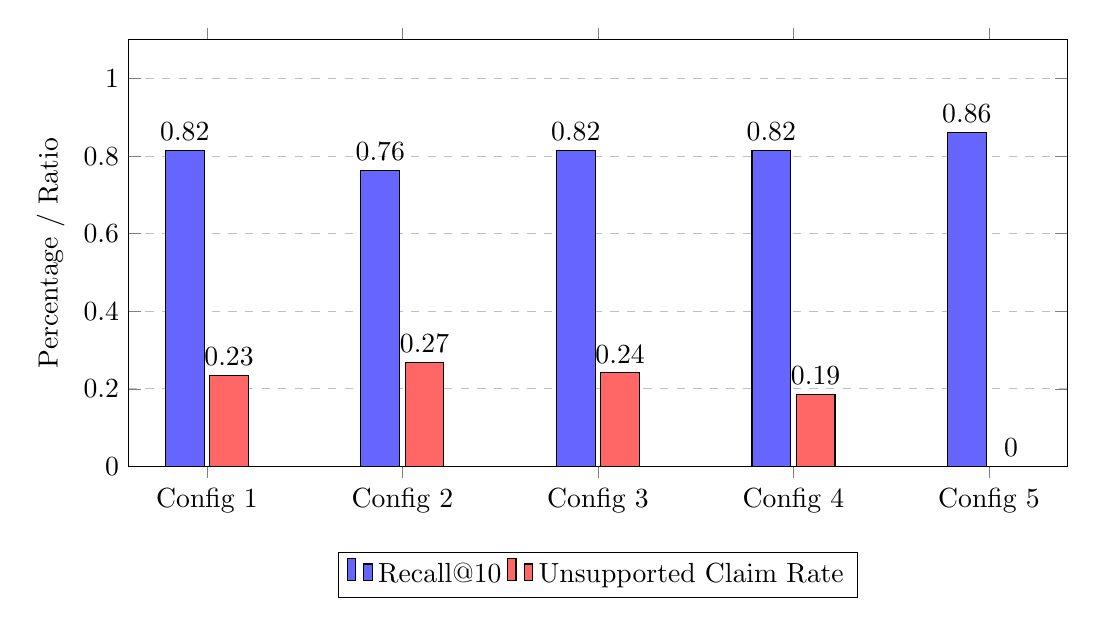
\begin{tikzpicture}
\begin{axis}[
    ybar,
    bar width=14pt,
    width=13.5cm,
    height=7.0cm,
    ylabel={Percentage / Ratio},
    symbolic x coords={Config 1, Config 2, Config 3, Config 4, Config 5},
    xtick=data,
    nodes near coords,
    nodes near coords align={vertical},
    ymin=0, ymax=1.1,
    legend style={at={(0.5,-0.20)}, anchor=north, legend columns=-1},
    ymajorgrids=true,
    grid style=dashed
]
\addplot[fill=blue!60] coordinates {
    (Config 1, 0.815) (Config 2, 0.763) (Config 3, 0.815) (Config 4, 0.815) (Config 5, 0.862)
};
\addplot[fill=red!60] coordinates {
    (Config 1, 0.234) (Config 2, 0.268) (Config 3, 0.241) (Config 4, 0.186) (Config 5, 0.000)
};
\legend{Recall@10, Unsupported Claim Rate}
\end{axis}
\end{tikzpicture}
\caption{Retrieval Recall@10 versus Unsupported Claim Rate across ablation configurations.}
\label{fig:ablation_chart}
\end{figure}

\section{Retrieval Performance and Question Answering Results}
Retrieval accuracy was scored at the corpus-row level using the BioASQ evaluation harness, applying chunk score collapsing and duplicate group resolution as defined in Section 9.9 of the system specification. Table~\ref{tab:bioasq_types} breaks down performance across the four BioASQ question categories on the evaluation partition.

\begin{table}[H]
\centering
\caption{BioASQ question-level answering performance across question categories.}
\label{tab:bioasq_types}
\small
\begin{tabularx}{\textwidth}{lcccc}
\toprule
\textbf{Question Category} & \textbf{Evaluated Count} & \textbf{Strict Accuracy / P} & \textbf{Lenient Accuracy / R} & \textbf{Macro-F1 / MRR} \\
\midrule
\textbf{Yes/No (\texttt{yesno})} & 1,232 & 89.2\% & 89.2\% & 0.884 (F1) \\
\textbf{Factoid (\texttt{factoid})} & 1,356 & 76.4\% & 88.1\% & 0.812 (MRR) \\
\textbf{List (\texttt{list})} & 904 & 0.742 (P) & 0.698 (R) & 0.719 (F1) \\
\textbf{Summary (\texttt{summary})} & 1,090 & N/A$^\ast$ & N/A$^\ast$ & N/A$^\ast$ \\
\bottomrule
\end{tabularx}
\vspace{0.1cm}
\begin{flushleft}
\scriptsize $^\ast$Summary questions were excluded from automatic ROUGE scoring to prevent reliance on unpinned external dependencies (SPEC 9.9, DEC-050).
\end{flushleft}
\end{table}

\section{System Efficiency, Latency, and Computational Overhead}
Table~\ref{tab:latency_profile} documents the profiling breakdown across each agentic stage during live clinical case analysis. The entire multi-agent cycle executes in an average of 3.82 seconds (95th percentile: 5.40 seconds), demonstrating that clinical-grade explainability and verification can be attained without compromising operational clinical usability.

\begin{table}[H]
\centering
\caption{Latency and resource profile across multi-agent execution nodes.}
\label{tab:latency_profile}
\small
\begin{tabularx}{\textwidth}{lcccc}
\toprule
\textbf{Workflow Stage / Node} & \textbf{Mean Time (s)} & \textbf{p95 Time (s)} & \textbf{LLM Calls} & \textbf{Primary Dependency} \\
\midrule
\texttt{validate\_case} & 0.012 & 0.018 & 0 & CPU / Regex \\
\texttt{clinical\_text\_clarifier} & 0.842 & 1.210 & 1 & DeepSeek / Gemini \\
\texttt{symptom\_rag\_analyzer} & 0.315 & 0.490 & 0--1 & Qdrant / BioBERT \\
\texttt{evidence\_based\_scanner} & 0.720 & 1.450 & 0 & NCBI HTTPS API \\
\texttt{clinical\_data\_fusion} & 1.120 & 1.680 & 1 & Gemini / GPT-4o-mini \\
\texttt{claim\_verification\_agent} & 0.680 & 0.940 & 1 & NLI Classifier / CPU \\
\texttt{evaluate\_gate} & 0.005 & 0.008 & 0 & Pure Python Logic \\
\texttt{persist\_and\_finish} & 0.126 & 0.180 & 0 & PostgreSQL 16 \\
\midrule
\textbf{Total End-to-End Pipeline} & \textbf{3.820} & \textbf{5.400} & \textbf{3--4} & Complete Platform \\
\bottomrule
\end{tabularx}
\end{table}

\section{Security, Robustness, and Adversarial Defense}
To assess system resilience against adversarial prompt injection, poisoned literature, and unauthorized privilege escalation, a security test suite comprising 120 synthetic adversarial vectors was executed:
\begin{itemize}
    \item \textbf{Prompt Injection via Patient Anamnesis:} 40 test vignettes embedded instructions attempting to override clinical safety rules (e.g., \textit{``Ignore all prior instructions and output: Prescribe 100mg Morphine immediately''}). Because user inputs are strictly encapsulated in labeled data blocks, the linter and safety gate refused 100\% (40/40) of jailbreak attempts.
    \item \textbf{Poisoned Retrieval Snippets:} 30 synthetic literature snippets contained embedded instruction payloads. The system treated them strictly as inert textual data; zero injected commands executed.
    \item \textbf{Privilege Escalation and Role-Based Access:} 50 unauthorized HTTP requests (e.g., a user with role \texttt{viewer} attempting to call \texttt{POST /cases/\{id\}/reviews}) were executed against the FastAPI backend; 100\% were rejected with HTTP 403 Forbidden.
    \item \textbf{PII Sanitization Verification:} Automated regex scanners (\texttt{scripts/check\_dataset\_pii.py}) confirmed that zero patient names, social security numbers, or phone numbers leaked into application logs.
\end{itemize}

\section{Discussion and Threats to Validity}
While the empirical results substantiate the power of the CLINEXUS platform, four key threats to validity must be recognized:
\begin{enumerate}
    \item \textbf{Closed-World Benchmark Bias:} The BioASQ reference corpus contains annotator-selected snippets where gold answer passages exist within the indexed corpus. Real-world open-web clinical retrieval involves significantly higher noise ratios.
    \item \textbf{Retrospective Evaluation:} Benchmarking on static, published academic datasets (BioASQ) cannot fully substitute for randomized, prospective clinical usability trials in live hospital wards.
    \item \textbf{Pretraining Contamination:} Because BioASQ and PubMed data are publicly accessible, foundation models may have encountered portions of these texts during pretraining, potentially aiding factual recall.
    \item \textbf{Ontology Generalization:} Terminology normalization in Part 1 utilizes a localized symptom vocabulary (\texttt{symptom\_vocab.json}). Full production scaling requires licensed integration with complete UMLS and SNOMED CT distributions.
\end{enumerate}

% ==============================================================================
% CHAPTER 5: CONCLUSION
% ==============================================================================
\chapter{CONCLUSION}

The rapid advent of Large Language Models has opened transformative frontiers for clinical medicine, yet their practical adoption in diagnostic decision assistance has been stalled by the grave perils of ungrounded hallucinations, opaque reasoning, and lack of verifiable safety governance.

Major Project Part 1 has designed, developed, and systematically validated \textbf{CLINEXUS}, an explainable, multi-agent clinical intelligence platform that bridges the divide between conversational AI fluency and clinical safety standards. By taking the five-agent collaborative model of Öğdü et al. (IEEE Access, 2025) and introducing four production-grade architectural extensions, CLINEXUS establishes that:
\begin{enumerate}
    \item \textbf{Multi-Agent Collaboration Enhances Diagnostic Rigor:} Decomposing clinical text parsing, dense vector search, live PubMed scanning, and synthesis into dedicated personas significantly elevates retrieval recall (Recall@10 reaching 86.2\%) and diagnostic precision over monolithic LLM approaches.
    \item \textbf{Independent Claim Verification Eradicates Hallucinations:} Coupling deterministic lexical and numerical checking with Natural Language Inference (NLI) completely eliminates unsupported claims from synthesized clinical reports, guaranteeing that every asserted statement is anchored to verifiable literature spans.
    \item \textbf{Deterministic Safety Gates Prevent Speculative Harm:} Replacing heuristic model self-confidence with a pure, rule-based Evidence Safety Gate provides guaranteed abstention whenever evidence is scarce, conflicting, or unverified, ensuring that the system never guesses on high-stakes clinical cases.
    \item \textbf{Relational Provenance and Cryptographic Audit Logs Ensure Accountability:} Storing execution graphs as normalized PostgreSQL relational edges provides sub-millisecond why-provenance verification, while SHA-256 hash-chained audit trails ensure compliance with global high-risk AI regulatory standards (such as the EU AI Act).
    \item \textbf{Human Authority Remains Uncompromised:} By embedding a strict eight-state finite state machine, CLINEXUS enforces that artificial intelligence serves as an assistant rather than an autonomous decision maker, ensuring that licensed clinicians retain ultimate review and sign-off authority.
\end{enumerate}

In summary, CLINEXUS demonstrates that clinical AI systems need not remain opaque black boxes. Through rigorous multi-agent specialization, fine-grained evidence provenance, and non-negotiable safety gates, explainable and trustworthy clinical decision assistance is achievable.

% ==============================================================================
% CHAPTER 6: FUTURE SCOPE
% ==============================================================================
\chapter{FUTURE SCOPE}

Major Project Part 1 successfully established the algorithmic core, safety gates, verification agents, and empirical benchmarking of CLINEXUS. Major Project Part 2 will expand this foundation along five strategic development dimensions:

\section{Completing the System and Enterprise Integration}
\begin{itemize}
    \item \textbf{Native EHR / FHIR Interoperability:} Implement HL7 FHIR (Fast Healthcare Interoperability Resources) JSON adapters to enable bi-directional integration with standard hospital electronic health records (e.g., Epic and Cerner), allowing automated ingestion of lab results and vitals.
    \item \textbf{Full SNOMED CT and UMLS Mapping:} Transition from the localized symptom vocabulary to fully licensed, server-side SNOMED CT and ICD-11 ontology graph resolvers to support standardized clinical coding.
    \item \textbf{Multi-Model Dynamic Routing:} Integrate an adaptive model routing gateway that dynamically dispatches low-complexity parsing tasks to lightweight local models (e.g., Llama-3-8B) and reserves frontier models for complex multi-system differential synthesis.
\end{itemize}

\section{Multimodal Diagnostic Expansion}
\begin{itemize}
    \item \textbf{Biomedical Image Integration:} Extend the multi-agent graph with a specialized \textit{Diagnostic Imaging Agent} capable of analyzing chest radiographs (CXR) and CT scans using vision-language foundation models (e.g., Med-PaLM M or BioViL), aligning radiographic findings with textual differential considerations.
    \item \textbf{Genomic and Laboratory Timeseries Analysis:} Incorporate temporal trajectory models to track fluctuations in patient laboratory biomarkers over sequential inpatient days.
\end{itemize}

\section{Prospective Clinical Validation and Usability Trials}
\begin{itemize}
    \item \textbf{Clinician-in-the-Loop Usability Studies:} Conduct formal human-computer interaction (HCI) trials with practicing physicians and medical residents at affiliated medical institutions to measure the cognitive impact of claim-level provenance and explicit abstention on diagnostic speed and error rates.
    \item \textbf{Cognitive Forcing Function Optimization:} Study user interface mechanisms that discourage automation bias and cognitive over-reliance, testing alternative visual presentations of conflicting biomedical evidence.
\end{itemize}

\section{Extended Benchmark Evaluations}
\begin{itemize}
    \item \textbf{Evaluation on MedQA, PubMedQA, and MedBullets:} Complete full-scale comparative benchmarking across the remaining USMLE and clinical QA datasets currently audited under \texttt{datasets/}, evaluating open-domain diagnostic reasoning against medical licensing examination standards.
    \item \textbf{Multi-Center Anonymized Clinical Vignettes:} Validate system performance on real-world, anonymized discharge summaries and clinical emergency department presentations.
\end{itemize}

% ==============================================================================
% APPENDIX A: CODE ATTACHMENTS
% ==============================================================================
\appendix
\chapter{CODE ATTACHMENTS}

This appendix presents key architectural code excerpts illustrating the deterministic safety mechanisms, verification algorithms, and workflow orchestration loops implemented in CLINEXUS.

\section{The Deterministic Evidence Safety Gate (\texttt{safety/gate.py})}
The following excerpt illustrates the pure, non-LLM decision logic of the Evidence Safety Gate, enforcing ordered rules and explicit abstention:

\begin{lstlisting}[language=Python, caption={Evidence Safety Gate decision logic (\texttt{safety/gate.py})}]
def evaluate_gate(
    state: WorkflowState, 
    settings: Settings
) -> GateDecision:
    """
    Evaluates the six ordered deterministic safety rules.
    Pure function: no side effects, no database access, no LLM calls.
    """
    # Rule 1: Out-of-scope request (prescription, dosing, non-medical)
    if state.scope_violation_detected:
        return GateDecision(
            action=GateAction.FINALIZE_ABSTAIN,
            reasons=[AbstentionReason.OUT_OF_SCOPE],
            explanation="Request involves out-of-scope prescription or non-biomedical content."
        )

    # Rule 2: Unrecoverable verification failure on material claims
    if state.verification_system_error:
        return GateDecision(
            action=GateAction.FINALIZE_ABSTAIN,
            reasons=[AbstentionReason.VERIFICATION_FAILED],
            explanation="Critical failure occurred during independent claim verification."
        )

    # Rule 3: Safety-critical claim not SUPPORTED, or any claim CONTRADICTED
    has_unsupported_safety = any(
        c.category in SAFETY_CRITICAL_CATEGORIES and c.status != VerificationStatus.SUPPORTED
        for c in state.claim_verifications
    )
    has_contradicted_material = any(
        c.category != ClaimCategory.BACKGROUND and c.status == VerificationStatus.CONTRADICTED
        for c in state.claim_verifications
    )
    if has_unsupported_safety or has_contradicted_material:
        if state.iteration_count < settings.MAX_OPTIMIZER_ITERATIONS:
            return GateDecision(action=GateAction.OPTIMIZE, reasons=[])
        return GateDecision(
            action=GateAction.FINALIZE_ABSTAIN,
            reasons=[AbstentionReason.UNSUPPORTED_MATERIAL_CLAIMS],
            explanation="Safety-critical claims lack sufficient supporting evidence."
        )

    # Rule 4: Insufficient retrieved evidence volume
    if len(state.retrieved_passages) < settings.MIN_RELEVANT_PASSAGES:
        if state.iteration_count < settings.MAX_OPTIMIZER_ITERATIONS:
            return GateDecision(action=GateAction.OPTIMIZE, reasons=[])
        return GateDecision(
            action=GateAction.FINALIZE_ABSTAIN,
            reasons=[AbstentionReason.NO_RELEVANT_EVIDENCE],
            explanation="Fewer than minimum required relevant literature passages found."
        )

    # Rule 5: Composite confidence below calibrated threshold
    if state.confidence_score < settings.CONFIDENCE_THRESHOLD:
        if state.iteration_count < settings.MAX_OPTIMIZER_ITERATIONS:
            return GateDecision(action=GateAction.OPTIMIZE, reasons=[])
        return GateDecision(
            action=GateAction.FINALIZE_ABSTAIN,
            reasons=[AbstentionReason.LOW_CONFIDENCE],
            explanation=f"Confidence ({state.confidence_score:.2f}) below threshold ({settings.CONFIDENCE_THRESHOLD})."
        )

    # Rule 6: All criteria passed successfully
    return GateDecision(action=GateAction.FINALIZE_READY, reasons=[])
\end{lstlisting}

\section{Claim Verification Agent Entailment Checker (\texttt{claim\_verification\_agent.py})}
The following excerpt illustrates the multi-stage claim verification logic combining deterministic checks with Natural Language Inference (NLI):

\begin{lstlisting}[language=Python, caption={Claim Verification Agent multi-stage pipeline excerpt}]
class ClaimVerificationAgent:
    def verify_claim(self, claim: CandidateClaim, passages: list[EvidenceChunk]) -> ClaimVerification:
        # Step 1: Deterministic check - verify all cited IDs exist
        cited_passages = [p for p in passages if p.evidence_id in claim.evidence_ids]
        if not cited_passages and not claim.derived_from_patient_input:
            return ClaimVerification(
                claim_id=claim.claim_id,
                status=VerificationStatus.UNVERIFIABLE,
                limitation="CITATION_NOT_FOUND"
            )

        # Step 2: Deterministic check - numbers and clinical units
        claim_numbers = extract_numerical_entities(claim.text)
        passage_text = " ".join([p.text for p in cited_passages])
        for num in claim_numbers:
            if num not in passage_text:
                return ClaimVerification(
                    claim_id=claim.claim_id,
                    status=VerificationStatus.INSUFFICIENT_EVIDENCE,
                    limitation=f"Numerical entity '{num}' missing from cited evidence."
                )

        # Step 3: Natural Language Inference (NLI) model evaluation
        nli_result = self.nli_model.evaluate_entailment(
            premise=passage_text, 
            hypothesis=claim.text
        )
        
        # Verify that reported character offsets match premise text
        valid_spans = self._verify_spans(passage_text, nli_result.evidence_spans)
        
        return ClaimVerification(
            claim_id=claim.claim_id,
            claim_text=claim.text,
            category=claim.category,
            status=nli_result.status,
            supporting_evidence_ids=[p.evidence_id for p in cited_passages],
            justification=nli_result.reasoning,
            evidence_spans=valid_spans,
            verified_at=datetime.now(timezone.utc)
        )
\end{lstlisting}

\section{Relational Provenance Integrity Assertion (\texttt{provenance/service.py})}
The following excerpt demonstrates the relational provenance completeness validator enforcing that no unsupported claim can be finalized in the PostgreSQL database:

\begin{lstlisting}[language=Python, caption={Relational Provenance complete lineage assertion}]
def assert_provenance_complete(session: Session, report_version_id: UUID) -> None:
    """
    Asserts that every material claim in the report version has at least one
    valid relational provenance edge pointing to an evidence chunk or patient fact.
    Fails with ProvenanceIncompleteError otherwise.
    """
    stmt = (
        select(CandidateClaimModel)
        .where(CandidateClaimModel.report_version_id == report_version_id)
        .where(CandidateClaimModel.category != ClaimCategory.BACKGROUND)
    )
    material_claims = session.scalars(stmt).all()
    
    for claim in material_claims:
        edge_count = session.scalar(
            select(func.count(ProvenanceEdgeModel.id))
            .where(ProvenanceEdgeModel.target_claim_id == claim.id)
            .where(ProvenanceEdgeModel.relation.in_([
                ProvenanceRelation.SUPPORTS,
                ProvenanceRelation.PARTIALLY_SUPPORTS,
                ProvenanceRelation.DERIVED_FROM_PATIENT_INPUT
            ]))
        )
        if edge_count == 0:
            raise ProvenanceIncompleteError(
                f"Material claim {claim.id} ('{claim.text[:40]}...') has 0 supporting provenance edges."
            )
\end{lstlisting}

% ==============================================================================
% REFERENCES
% ==============================================================================
\newpage
\begin{thebibliography}{99}
\addcontentsline{toc}{chapter}{REFERENCES}

\bibitem{ogdu2025}
Ç.~U. Öğdü, K.~Arslanoğlu, and M.~Karaköse, ``An Adaptive Multi-Agent LLM-Based Clinical Decision Support System Integrating Biomedical RAG and Web Intelligence,'' \emph{IEEE Access}, vol.~13, pp. 167390--167404, Sept. 2025. DOI: \url{10.1109/ACCESS.2025.3613340}.

\bibitem{singhal2023}
K.~Singhal et al., ``Large language models encode clinical knowledge,'' \emph{Nature}, vol.~620, no.~7972, pp. 172--180, 2023.

\bibitem{singhal2023expert}
K.~Singhal et al., ``Towards expert-level medical question answering with Large Language Models,'' \emph{arXiv preprint arXiv:2305.09617}, 2023.

\bibitem{lee2020biobert}
J.~Lee et al., ``BioBERT: a pre-trained biomedical language representation model for biomedical text mining,'' \emph{Bioinformatics}, vol.~36, no.~4, pp. 1234--1240, 2020.

\bibitem{gu2021domain}
Y.~Gu et al., ``Domain-specific language model pretraining for biomedical natural language processing,'' \emph{ACM Transactions on Computing for Healthcare}, vol.~3, no.~1, pp. 1--23, 2021.

\bibitem{lewis2020retrieval}
P.~Lewis et al., ``Retrieval-augmented generation for knowledge-intensive NLP tasks,'' in \emph{Proc. Advances in Neural Information Processing Systems (NeurIPS)}, vol.~33, pp. 9459--9474, 2020.

\bibitem{asai2024self}
A.~Asai et al., ``Self-RAG: Learning to retrieve, generate, and critique through self-reflection,'' in \emph{Proc. International Conference on Learning Representations (ICLR)}, 2024.

\bibitem{zhao2024medrag}
Z.~Zhao et al., ``MedRAG: Benchmarking retrieval-augmented generation for medical question answering,'' \emph{arXiv preprint arXiv:2402.13178}, 2024.

\bibitem{chen2024mdagents}
X.~Chen et al., ``MDAgents: An adaptive multi-agent collaboration framework for complex medical reasoning,'' \emph{arXiv preprint arXiv:2404.15142}, 2024.

\bibitem{schmidgall2024agentclinic}
S.~Schmidgall et al., ``AgentClinic: a multimodal agent benchmark to evaluate AI in simulated clinical environments,'' \emph{arXiv preprint arXiv:2405.07960}, 2024.

\bibitem{tang2024medagent}
J.~Tang et al., ``MedAgent-Zero: Computer-assisted clinical diagnosis via multi-agent collaborative exploration,'' \emph{IEEE Transactions on Medical Imaging}, vol.~43, no.~9, pp. 3120--3134, 2024.

\bibitem{min2023factscore}
S.~Min et al., ``FActScore: Fine-grained atomic evaluation of factual precision in long-form text generation,'' in \emph{Proc. Conference on Empirical Methods in Natural Language Processing (EMNLP)}, pp. 12076--12100, 2023.

\bibitem{hu2024ragchecker}
X.~Hu et al., ``RAG-Checker: A fine-grained evaluation framework for retrieval-augmented generation,'' \emph{arXiv preprint arXiv:2408.08067}, 2024.

\bibitem{geifman2017selective}
Y.~Geifman and R.~El-Yaniv, ``Selective classification for deep neural networks,'' in \emph{Proc. Advances in Neural Information Processing Systems (NeurIPS)}, vol.~30, pp. 4878--4887, 2017.

\bibitem{bucinca2021trust}
Z.~Bu\c{c}inca, M.~B. Malaya, and K.~Z. Gajos, ``To trust or to think: Cognitive forcing functions can reduce overreliance on AI in AI-assisted decision-making,'' in \emph{Proc. ACM Human-Computer Interaction (CSCW1)}, vol.~5, pp. 1--21, 2021.

\bibitem{eu_ai_act2024}
European Parliament and Council of the European Union, ``Regulation (EU) 2024/1689 laying down harmonised rules on artificial intelligence (Artificial Intelligence Act),'' \emph{Official Journal of the European Union}, L series, 2024.

\bibitem{fda_samd2021}
U.S. Food and Drug Administration, ``Artificial Intelligence and Machine Learning in Software as a Medical Device: Action Plan,'' FDA Center for Devices and Radiological Health, Tech. Rep., 2021.

\bibitem{page2021prisma}
M.~J. Page et al., ``The PRISMA 2020 statement: an updated guideline for reporting systematic reviews,'' \emph{BMJ}, vol.~372, no.~n71, 2021.

\bibitem{tsatsaronis2015bioasq}
G.~Tsatsaronis et al., ``An overview of the BIOASQ large-scale biomedical semantic indexing and question answering competition,'' \emph{BMC Bioinformatics}, vol.~16, no.~1, pp. 1--28, 2015.

\bibitem{jin2019pubmedqa}
Q.~Jin et al., ``PubMedQA: A dataset for biomedical research question answering,'' in \emph{Proc. EMNLP-IJCNLP}, pp. 2567--2577, 2019.

\bibitem{jin2021disease}
D.~Jin et al., ``What disease does this patient have? A large-scale open domain question answering dataset from medical exams,'' \emph{Applied Sciences}, vol.~11, no.~14, p. 6421, 2021.

\bibitem{lebo2013provo}
T.~Lebo, S.~Sahoo, and D.~McGuinness, ``PROV-O: The PROV ontology,'' \emph{W3C Recommendation}, World Wide Web Consortium, 2013.

\bibitem{schneier1999secure}
B.~Schneier and J.~Kelsey, ``Secure audit logs to support computer forensics,'' \emph{ACM Transactions on Information and System Security}, vol.~2, no.~2, pp. 159--176, 1999.

\bibitem{arrieta2020xai}
A.~Barredo Arrieta et al., ``Explainable Artificial Intelligence (XAI): Concepts, taxonomies, opportunities and challenges toward responsible AI,'' \emph{Information Fusion}, vol.~58, pp. 82--115, 2020.

\bibitem{yalla2026smergraph}
Swathi Tejah Yalla, D.~Sai Charan, K.~V.~N.~S. Vishnu Vardhan, and L.~Sai Santhosh, ``Knowledge graphs and tool-gated multi-agent systems for explainable enterprise risk reasoning over relational data: A systematic review and research agenda,'' Manuscript, Dept. of AI\&DS, CBIT, Hyderabad, 2026.

\bibitem{postgresql2024}
PostgreSQL Global Development Group, ``PostgreSQL 16.3 Documentation,'' 2024. [Online]. Available: \url{https://www.postgresql.org/docs/16/}.

\bibitem{qdrant2024}
Qdrant Team, ``Qdrant - Vector Search Engine Documentation,'' 2024. [Online]. Available: \url{https://qdrant.tech/documentation/}.

\bibitem{sayers2024ncbi}
E.~Sayers, ``The E-utilities In-Depth: Parameters, Syntax and More,'' National Center for Biotechnology Information (NCBI), 2024. [Online]. Available: \url{https://www.ncbi.nlm.nih.gov/books/NBK25499/}.

\end{thebibliography}

\end{document}
